% Journal of Symbolic Computation (Elsevier) — elsarticle template.
% Compile: pdflatex -> bibtex -> pdflatex x2.  Bibliography style: elsarticle-num.
\documentclass[preprint,12pt]{elsarticle}
\usepackage[T1]{fontenc}\usepackage[utf8]{inputenc}
\usepackage{amsmath,amssymb,amsthm,mathtools}
\usepackage{booktabs,tabularx,array,graphicx}
\usepackage[hidelinks]{hyperref}\usepackage{url}
\graphicspath{{figures/}{../figures/}}
\setlength{\emergencystretch}{1.5em}
\newtheorem{thm}{Theorem}[section]\newtheorem{lem}[thm]{Lemma}\newtheorem{cor}[thm]{Corollary}\newtheorem{prop}[thm]{Proposition}
\theoremstyle{definition}\newtheorem{defi}[thm]{Definition}\newtheorem{prob}[thm]{Problem}\newtheorem{obs}[thm]{Observation}
\theoremstyle{remark}\newtheorem{rem}[thm]{Remark}
\newcommand{\ZZ}{\mathbb Z}\newcommand{\Sym}{\operatorname{Sym}}\newcommand{\Alt}{\operatorname{Alt}}
\newcommand{\ctype}{\operatorname{ctype}}\DeclareMathOperator{\Cent}{C}\DeclareMathOperator{\supp}{supp}
\newcommand{\Pthree}{\mathsf{P}_3}\newcommand{\Conj}[1]{\mathsf{Conj}_{#1}}\newcommand{\Dzero}{\Conj{3}}\newcommand{\TR}{T_{\mathcal R}}
\journal{Journal of Symbolic Computation}
\begin{document}
\begin{frontmatter}
\title{One-variable equations of length three over symmetric groups: normal forms, the hardness of conjugacy by an element of prescribed order, and layered permutation walks}
\author[a]{Gautier-Edouard Filardo}
\ead{gautier-edouard.filardo@efrei.fr}
\affiliation[a]{organization={Efrei Research Lab, Efrei Paris Panth\'eon-Assas},city={Villejuif},country={France}}
\begin{abstract}
We study the equation $x\,a\,x^{2}=c$ with unknown $x$ and constants $a,c$ in the symmetric group $\Sym(N)$, where $N$ is part of the input. Every one-variable word with at most two occurrences of the unknown reduces to root extraction or conjugacy and is decided in polynomial time from cycle types, and every word with three positive occurrences is equivalent to this one, so it is a shortest one-variable shape over permutation groups whose complexity is not classified. We prove that its restriction to solutions of order three -- equivalently, deciding whether two permutations are conjugate by an element of order three -- is NP-complete, already when $a$ has all cycles of one prime length and $c$ commutes with $a$; the reduction is from Numerical 3-Dimensional Matching and every certificate has cycle type $3^{N/3}$. More generally, conjugacy by an element of order $n$ is NP-complete for every $n\ge3$ and polynomial for $n=2$ (in time $O(N^{3})$, by pairing the orbits of $\langle a,c\rangle$), so the question ``does the coset of conjugators of $a$ to $c$ contain an element of order $n$'' is completely classified. Consequently the natural algorithm that enumerates the cycle type of the unknown cannot be polynomial per type unless $\mathrm P=\mathrm{NP}$. We give the polynomial special cases (bounded support of $a$, solutions commuting with $a$, pairs of involutions), an exact first-moment identity for the number of solutions, and a pair of permutations in $\Sym(7)$ generating $\mathrm{PSL}(2,7)$ for which every word in $a,c$ has the same cycle type and the same group data on both sides while one equation is solvable and the other is not -- the classical Gassmann pair of degree seven -- so no such invariant decides solvability. Conjugacy by an element of order three is exactly the system of the two equations $xax^{2}=c$, $xa^{2}x^{2}=c^{2}$, and we show that the natural paddings of this system into a single equation acquire spurious solutions; the complexity of a single equation remains open. Finally we show that the round of a two-register layered permutation walk proposed as a one-way function is exactly this equation in the wreath product $\Alt(m)\wr C_2$, and we measure the cost of constraint-propagation solvers, which grows as $|\Alt(m)|^{\Theta(1)}$; the resulting meet-in-the-middle attack costs between $2^{165}$ and $2^{196}$ at the parameters originally proposed. 
\end{abstract}
\begin{keyword}
permutation groups \sep equations in groups \sep NP-completeness \sep cycle types \sep conjugacy \sep elements of prime order \sep wreath products \sep one-way functions
\MSC[2020] 20B40 \sep 68Q17 \sep 20F10 \sep 94A60
\end{keyword}
\end{frontmatter}




\section{Introduction}

Let $\Sym(N)$ act on $[N]=\{0,\ldots,N-1\}$, with products read right to left, $(pq)(j)=p(q(j))$. A \emph{one-variable word} is a product $w(x)=c_0x^{\varepsilon_1}c_1x^{\varepsilon_2}\cdots x^{\varepsilon_\ell}c_\ell$ with constants $c_i\in\Sym(N)$ and $\varepsilon_i\in\{\pm1\}$; $\ell$ is its \emph{$x$-length}. We are interested in the decision problem
\[
 \text{given } a,c\in\Sym(N),\ \text{is there } x\in\Sym(N)\text{ with } x\,a\,x^{2}=c\,?
\]
which we call $\Pthree$. The group is part of the input: $N$ grows, the shape of the equation is fixed.

This regime differs from the classical one. Goldmann and Russell \cite{goldmann2002} classified the complexity of equation satisfiability over a \emph{fixed} finite group, with an unbounded number of variables and unbounded word length: polynomial for nilpotent groups, NP-complete for non-solvable ones; the solvable non-nilpotent case has since been narrowed under the exponential time hypothesis \cite{horvath2011,idziak2022,weiss2020}. When instead the group is a permutation group given by generators, membership is polynomial by Schreier--Sims \cite{sims1970,seress2003,luks1993}, while a number of natural refinements are NP-complete: containing a fixed-point-free element or an element of a prescribed cycle type \cite{lubiw1981,cameronwu2010,arvind2013}, subgroup distance \cite{buchheim2009}, knapsack and subset-sum variants \cite{lohrey2022mfcs,lohrey2025membership}, spherical (multi-variable quadratic) equations $z_1^{-1}g_1z_1\cdots z_k^{-1}g_kz_k=1$ over $\Sym(N)$ and $\Alt(N)$ with $N$ in the input \cite{mattes2024spherical}, and, most recently, the cycle-type problem for groups generated by two commuting permutations and for cosets of cyclic groups \cite{lohreyrosowski2025}. Our problem has no generators in the input at all: its only data are two permutations, and its unknown ranges over the whole of $\Sym(N)$.

For one-variable words of small $x$-length over $\Sym(N)$ everything is easy. Length one is a single equation $x^{\pm1}=c'$; length two is square-root extraction or conjugacy (Proposition~\ref{prop:short}). Length three is the first case where the classical invariants fail, and all positive words of length three are one problem (Proposition~\ref{prop:three}). Word maps with constants on symmetric groups have been studied for their equidistribution and fibre statistics \cite{larsen2012,shalev2009,garion2009,schneider2023,alekseev2025}; those results explain the statistics of the solution set (Section~\ref{sec:stat}) but have no algorithmic content.

Our motivation came from cryptanalysis. A candidate one-way function of \cite{filardo2026cpwi} iterates, over the alternating group $\Alt(m)$, a two-register recurrence $U'=UAVU$, $V'=VBUV$ whose constants $(A,B)$ are selected by the input bits; inverting $n$ rounds is exactly $n$ instances of the single-round system, and we show (Theorem~\ref{thm:wreath}) that the single-round system \emph{is} $\Pthree$ inside the wreath product $\Alt(m)\wr C_2\le\Sym(2m)$. The security of that construction therefore rests on the complexity of $\Pthree$, which is why we set out to classify it. The pattern is familiar from group-based cryptography, where the hardness of a construction reduced to an equation whose structure was then exploited: Euclidean structure in $\mathrm{SL}_2$ for the Tillich--Z\'emor and LPS hash functions \cite{tillich1994,petit2008,grassl2011}, linear representations for braid-group conjugacy \cite{cheon2003,myasnikov2005,tsaban2015}. No such structure is available here: equations over free groups have a rich theory \cite{lyndon1960}, but $\Sym(N)$ with $N$ in the input is neither fixed nor free.

\paragraph{Results.} We did not classify $\Pthree$, but we located it precisely.
\begin{enumerate}
\item \emph{Short words} (Section~\ref{sec:short}). Every one-variable word of $x$-length at most two over $\Sym(N)$ is decided in polynomial time; every word with three positive occurrences of $x$ is polynomially equivalent to $\Pthree$, whose solution sets are in explicit bijection.
\item \emph{Structure} (Section~\ref{sec:struct}). $\Pthree$ is in NP and is polynomial when the support of $a$ is bounded, when only solutions commuting with $a$ are sought, and when $a$ and $c$ are involutions. Its solution count satisfies an exact first-moment identity, $\sum_{c\in\gamma}\#\{x:xax^{2}=c\}=\#\{x:\ctype(ax^{3})=\gamma\}$, whose right-hand side is a class-algebra quantity and has a closed form (Theorem~\ref{thm:firstmoment}). No invariant built from the cycle types of words in $a,c$ -- of any length -- or from the orbit structure, order, isomorphism type or permutation character of $\langle a,c\rangle$ decides solvability: two pairs in $\Sym(7)$ generating $\mathrm{PSL}(2,7)$ witness this (Theorem~\ref{thm:psl}). The equation is self-dual under $(a,c,x)\mapsto(c,a,x^{-1})$, and for $a$ an $N$-cycle and $c$ a transposition the solution count has an explicit $O(N)$ formula (Theorem~\ref{thm:transposition}).
\item \emph{Hardness} (Section~\ref{sec:hard}). Deciding whether two permutations are conjugate by an element of order three -- the restriction of $\Pthree$ to solutions with $x^{3}=1$ -- is NP-complete, already for $a$ with all cycles of one prime length $L\equiv2\pmod3$, for $c\in\Cent(a)$, and with certificates of cycle type $3^{N/3}$ (Theorem~\ref{thm:main}). Hence $\Pthree$ restricted to a prescribed cycle type of the unknown is polynomial for types with parts at most two and NP-complete for the type $3^{N/3}$, and no algorithm that enumerates the cycle type of $x$ can be polynomial per type unless $\mathrm P=\mathrm{NP}$ (Corollary~\ref{cor:noenum}). Conjugacy by an element of order $n$ is NP-complete for every $n\ge3$ and polynomial for $n=2$ (Theorems~\ref{thm:conjn} and~\ref{thm:conj2}), $\Dzero$ is exactly a system of two $\Pthree$ equations with a common unknown (Lemma~\ref{lem:twoeq}), and the natural paddings of this system into one equation acquire spurious solutions (Proposition~\ref{prop:fourlayer}).
\item \emph{Application} (Section~\ref{sec:cpwi}). The single-round system of the layered walk is $\Pthree$ in $\Alt(m)\wr C_2$; constraint-propagation solvers reach a planted solution after about $0.38\,m$ free decisions with domains of size about $m$, so their cost is $|\Alt(m)|^{\Theta(1)}$, and the resulting meet-in-the-middle attack costs between $2^{165}$ and $2^{196}$ at the parameters $(n,m)=(256,36)$ originally proposed -- below exhaustive search, above the $128$-bit target.
\end{enumerate}
Section~\ref{sec:open} lists what remains open. Every statement labelled ``verified'' was checked by exhaustive or randomised computation whose scripts and records accompany the paper.

\section{Short words}\label{sec:short}

We write $\ctype(p)$ for the cycle type of $p$ (a partition of $N$), $\Cent(p)$ for its centraliser, and $p\sim q$ for conjugacy. Two permutations are conjugate iff they have the same cycle type, and a conjugator is found in linear time; the conjugators form a coset of $\Cent(p)$.

\begin{prop}[$x$-length at most two]\label{prop:short}
Every one-variable equation $w(x)=c$ of $x$-length at most two over $\Sym(N)$ is decided, and a solution produced, in polynomial time.
\end{prop}
\begin{proof}
After multiplying by the outer constants, a word of $x$-length one is $x^{\pm1}=c'$. A word of $x$-length two is $x^{\varepsilon_1}c_1x^{\varepsilon_2}=c'$. If $\varepsilon_1=-\varepsilon_2$ it is the conjugacy $x^{\mp1}c_1x^{\pm1}=c'$, decided by $\ctype(c_1)=\ctype(c')$. If $\varepsilon_1=\varepsilon_2=1$ then $xc_1x=c'$ is equivalent to $(xc_1)^{2}=c'c_1$: $y=xc_1$ is a square root of $c'c_1$, which exists iff, for every even $m$, the number of $m$-cycles of $c'c_1$ is even \cite{blum1974}, and then $x=yc_1^{-1}$. If $\varepsilon_1=\varepsilon_2=-1$, invert both sides.
\end{proof}

\begin{prop}[positive words of $x$-length three]\label{prop:three}
For constants $a,b,c$ the equation $x\,a\,x\,b\,x=c$ has the same number of solutions as $z\,e\,z^{2}=f$ with $e=b^{-1}a$ and $f=(ca)^{-1}$, via the bijection $z=(xa)^{-1}$. Every one-variable word with three positive occurrences of $x$ is therefore polynomially equivalent to $\Pthree$ (for the symmetry
$(a,c,x)\mapsto(c,a,x^{-1})$ of $\Pthree$ itself see Proposition~\ref{prop:dual}).
\end{prop}
\begin{proof}
Put $y=xa$. Then $xaxbx=y\,(ya^{-1})\,b\,(ya^{-1})=y^{2}(a^{-1}b)\,y\,a^{-1}$, so the equation reads $y^{2}(a^{-1}b)y=ca$; inverting both sides and putting $z=y^{-1}$ gives $z\,(a^{-1}b)^{-1}z^{2}=(ca)^{-1}$. A general positive word $c_0xc_1xc_2xc_3=c$ is of this form after multiplying by $c_0^{-1}$ and $c_3^{-1}$. 
\end{proof}

\begin{rem}
Words of $x$-length three with mixed signs, such as $x\,a\,x\,b\,x^{-1}=c$, are not covered by Proposition~\ref{prop:three}; they are a distinct family that we do not treat here.
\end{rem}

Two elementary reformulations are used throughout.
\begin{lem}[conjugation form]\label{lem:conj}
$x\,a\,x^{2}=c$ if and only if $x^{-1}cx=a\,x^{3}$. In particular every solution satisfies $\ctype(a\,x^{3})=\ctype(c)$, and, writing $b=xax^{-1}$, one has $c=b\,x^{3}$, i.e.\ $x^{3}=b^{-1}c$ with $b\sim a$.
\end{lem}
\begin{proof}
Multiply $xax^{2}=c$ on the left by $x^{-1}$ and on the right by $x$; the second form is $c=(xax^{-1})x^{3}$.
\end{proof}

\section{Structure of the solution set}\label{sec:struct}

\subsection{Polynomial special cases}

\begin{lem}[cube roots of a permutation]\label{lem:cuberoots}
Let $t\in\Sym(N)$. A permutation $x$ with $x^{3}=t$ permutes the cycles of $t$, and the $x$-orbits of cycles have size $1$ or $3$. The cube roots of $t$ are in bijection with the following data:
a partition of the set of cycles of $t$ into \emph{singletons}, which must have length $\ell\not\equiv0\pmod 3$, and \emph{triples} of cycles of a common length $\ell$ (any $\ell$);
on a singleton $D$ of length $\ell$ one has $x|_{D}=t^{k}|_{D}$ with $3k\equiv1\pmod\ell$ (one choice);
on a triple $\{D_1,D_2,D_3\}$ the restriction of $x$ is one of exactly $2\ell^{2}$ permutations of $D_1\cup D_2\cup D_3$, namely those obtained by choosing a cyclic order $D_{1}\to D_{i}\to D_{j}\to D_{1}$ ($2$ choices), the image $x(p_1)\in D_i$ of a fixed base point $p_1\in D_1$ ($\ell$ choices) and the image $x(x(p_1))\in D_j$ ($\ell$ choices), and extending by $x(t^{u}q)=t^{u}x(q)$ and $x^{3}=t$.
Consequently, if $t$ has $n_\ell$ cycles of length $\ell$, the number of cube roots of $t$ is
\begin{equation}\label{eq:cuberootcount}
\prod_{\ell\ge1}\ \sum_{k=0}^{\lfloor n_\ell/3\rfloor}\frac{n_\ell!}{k!\,6^{k}\,(n_\ell-3k)!}\,(2\ell^{2})^{k}\,\sigma_\ell^{\,n_\ell-3k},
\qquad \sigma_\ell=\begin{cases}1&3\nmid\ell,\\0&3\mid\ell,\end{cases}
\end{equation}
with the convention $0^{0}=1$; in particular $t$ has a cube root iff $3\mid n_\ell$ for every $\ell\equiv0\pmod 3$.
\end{lem}
\begin{proof}
Since $x$ commutes with $t=x^{3}$, it maps $t$-cycles onto $t$-cycles of the same length; the induced permutation $\bar x$ of the cycles satisfies $\bar x^{3}=\bar t=\mathrm{id}$, so its orbits have size $1$ or $3$.
If $D$ is a fixed cycle of $\bar x$ then $x|_D$ commutes with the $\ell$-cycle $t|_D$ and lies in its centraliser $\langle t|_D\rangle$ (a transitive cyclic group is self-centralising), so $x|_D=t^{k}|_D$ with $t^{3k}=t$ on $D$, i.e.\ $3k\equiv1\pmod\ell$: this has a (unique) solution iff $3\nmid\ell$.
If $\{D_1,D_2,D_3\}$ is an orbit of size $3$, say $x(D_1)=D_i$, $x(D_i)=D_j$, the three cycles have the same length $\ell$ and $x$ is determined on $D_1$ by $x(p_1)$ (because $x(t^{u}p_1)=t^{u}x(p_1)$), on $D_i$ by $x(x(p_1))$, and on $D_j$ by $x^{3}=t$, i.e.\ $x(x^{2}(t^{u}p_1))=t^{u+1}p_1$; conversely every such choice defines a bijection of $D_1\cup D_i\cup D_j$ which commutes with $t$ on each of the three cycles by construction, and whose cube is $t$: it is $t$ on $D_1$ by construction, and since $x^{3}$ commutes with $x$, $x^{3}(x(q))=x(x^{3}(q))=x(t(q))=t(x(q))$ for $q\in D_1$, so $x^{3}=t$ on $x(D_1)$ and likewise on $x^{2}(D_1)$. This gives $2\cdot\ell\cdot\ell$ roots per triple, independent of the ordering of the triple.
The count~\eqref{eq:cuberootcount} follows: $n!/(k!\,6^{k}(n-3k)!)$ is the number of ways to choose $k$ disjoint unordered triples among $n$ labelled cycles.
\end{proof}

\begin{lem}[cube roots with prescribed images]\label{lem:prescribed}
Given $t\in\Sym(N)$ and a partial injection $f\colon S\to[N]$, the number of $x\in\Sym(N)$ with $x^{3}=t$ and $x|_{S}=f$ is computed in time $O(N)$ after the cycle decomposition of $t$ (in particular, existence is decided in polynomial time).
\end{lem}
\begin{proof}
Let $D(q)$ denote the $t$-cycle of a point $q$ and $\ell(D)$ the length of a cycle $D$. We encode the constraints as a directed graph $\Gamma$ on the cycles of $t$: for each $p\in S$ put an edge $D(p)\to D(f(p))$ labelled by the \emph{phase} $d\in\ZZ_{\ell}$ defined by $f(p)=t^{d}(q_{0})$ where $q_0$ is a fixed base point of $D(f(p))$ and $p=t^{u}(p_0)$ with $p_0$ the base point of $D(p)$; precisely $d=\mathrm{pos}(f(p))-\mathrm{pos}(p)\bmod\ell$, so that $x|_{D(p)}$ is forced to be $t^{u}p_0\mapsto t^{u+d}q_0$. By Lemma~\ref{lem:cuberoots} a root $x$ with $x|_S=f$ exists only if:
\begin{enumerate}
\item[(i)] $\ell(D(p))=\ell(D(f(p)))$ for all $p\in S$ ($x$ preserves lengths);
\item[(ii)] two points $p,p'\in S$ on the same cycle give the same edge (same target cycle and same phase), since $x|_{D(p)}$ is determined by one image;
\item[(iii)] no two distinct cycles have edges to the same target ($\bar x$ is a bijection).
\end{enumerate}
When (i)--(iii) hold, every vertex of $\Gamma$ has in- and out-degree at most one, so the connected components of $\Gamma$ are directed paths and directed cycles; moreover, since $\bar x^{3}=\mathrm{id}$, the component containing a touched cycle $D$ is contained in the $\bar x$-orbit of $D$, which has size $1$ or $3$. Hence a root exists only if every component is one of:
\begin{enumerate}
\item[(a)] a loop $D\to D$: then $D$ is a singleton, which requires $3\nmid\ell(D)$ and phase $d\equiv k\pmod\ell$ with $3k\equiv1$ (one root restricted to $D$, or none);
\item[(b)] a directed $3$-cycle $D_1\to D_2\to D_3\to D_1$ with phases $d_1,d_2,d_3$: it is a complete triple; the composite $D_1\to D_1$ is $t^{d_1+d_2+d_3}$ and must equal $t$, i.e.\ $d_1+d_2+d_3\equiv1\pmod\ell$ (one root restricted to the triple, or none);
\item[(c)] a path with two edges $D_1\to D_2\to D_3$: it is the triple $\{D_1,D_2,D_3\}$, and $x|_{D_3}$ is determined by $x^{3}=t$; exactly one root restricted to the triple;
\item[(d)] a path with one edge $D_1\to D_2$: the triple must be completed by a third cycle $D_3$ of length $\ell=\ell(D_1)$ which is \emph{free}, i.e.\ isolated in $\Gamma$ (every touched cycle already carries an edge and belongs to another component); given $D_3$ there are $\ell$ choices for $x(x(p_1))\in D_3$, after which $x$ is determined on the triple.
\end{enumerate}
Components of any other shape (a directed $2$-cycle, a cycle of length $\ge4$, a path with $\ge3$ edges) are incompatible with $\bar x^{3}=\mathrm{id}$ and give no root. Conversely, suppose (i)--(iii) hold, every component is of type (a)--(d) with the stated congruences, and let $n_\ell$ be the number of free cycles of length $\ell$ and $q_\ell$ the number of components of type (d) of length $\ell$. A root $x$ with $x|_S=f$ is then exactly: a choice, for the $q_\ell$ components of type (d), of distinct free third cycles and phases, $n_\ell(n_\ell-1)\cdots(n_\ell-q_\ell+1)\,\ell^{\,q_\ell}$ possibilities, together with an arbitrary cube root (Lemma~\ref{lem:cuberoots}) of $t$ restricted to the $n_\ell-q_\ell$ remaining free cycles, for each $\ell$. Therefore the number of roots is
\begin{equation}\label{eq:prescribedcount}
\prod_{\ell}\ (n_\ell)_{q_\ell}\,\ell^{\,q_\ell}\ \sum_{k}\frac{(n_\ell-q_\ell)!}{k!\,6^{k}\,(n_\ell-q_\ell-3k)!}\,(2\ell^{2})^{k}\,\sigma_\ell^{\,n_\ell-q_\ell-3k},
\end{equation}
(falling factorial $(n)_q$; the product is $0$ if some $n_\ell<q_\ell$, or if some component violates (a)--(d)); in particular a root exists iff (i)--(iii) hold, all components are of type (a)--(d) with the stated congruences, $n_\ell\ge q_\ell$ for all $\ell$, and $n_\ell-q_\ell\equiv0\pmod 3$ for every $\ell\equiv0\pmod3$. Building $\Gamma$ and checking all conditions takes $O(N)$ operations once the cycles of $t$ are known.
\end{proof}

\begin{lem}[bounded support]\label{lem:support}
If $|\supp(a)|=s$, the number of solutions of $x\,a\,x^{2}=c$ is computed, and in particular $\Pthree$ is decided, in time $O(N^{s+1})$, hence $N^{O(s)}$.
\end{lem}
\begin{proof}
Let $S=\supp(a)$, $|S|=s$. By Lemma~\ref{lem:conj}, $x$ is a solution iff $c=b\,x^{3}$ with $b=xax^{-1}$. The permutation $b$ is determined by $f:=x|_{S}$: $\supp(b)=f(S)$ and $b(f(p))=f(a(p))$ for $p\in S$; write $b=b_f$. Conversely, let $f\colon S\to[N]$ be any injection, $b_f$ the permutation just described (it is well defined because $a(S)=S$), and $t_f=b_f^{-1}c$. If $x^{3}=t_f$ and $x|_S=f$, then $xax^{-1}$ agrees with $b_f$ on $f(S)=x(S)$ and is the identity off $x(S)$, so $xax^{-1}=b_f$ and $c=b_f t_f=xax^{-1}x^{3}=xax^{2}$. Hence
\[
\{x:\ xax^{2}=c\}\;=\;\bigsqcup_{f\colon S\hookrightarrow[N]}\{x:\ x^{3}=t_f,\ x|_{S}=f\},
\]
the union being disjoint since $f=x|_S$ is recovered from $x$. There are $N!/(N-s)!\le N^{s}$ injections $f$, and for each of them the cardinality of the right-hand set is computed in $O(N)$ time by Lemma~\ref{lem:prescribed}. Summing gives the number of solutions in $O(N^{s+1})$ time.
\end{proof}

\begin{lem}[solutions commuting with the constant]\label{lem:cent}
Let $a\in\Sym(N)$ have $m_L$ cycles of length $L$, so that $\Cent(a)\cong\prod_{L}\ZZ_L\wr\Sym(m_L)$. The solutions of $x\,a\,x^{2}=c$ that commute with $a$ are exactly the cube roots of $t=a^{-1}c$ lying in $\Cent(a)$; they exist only if $c\in\Cent(a)$. Suppose $c\in\Cent(a)$. For each $L$, $t$ permutes the $m_L$ cycles of $a$ of length $L$; let $\rho_L$ be this permutation of cycles, and for each $\rho_L$-cycle $\Delta$, of length $\ell$, define its \emph{rotation} $R(\Delta)\in\ZZ_L$ by $t^{\ell}|_{C}=a^{R(\Delta)}|_{C}$ for one (equivalently every) $a$-cycle $C\in\Delta$. Let $n_{L}(\ell,R)$ be the number of $\rho_L$-cycles of length $\ell$ and rotation $R$. Call the class $(L,\ell,R)$ \emph{free} if $3\nmid\ell$ and ($3\nmid L$ or $R\equiv0\pmod3$), and \emph{bound} otherwise. Then:
\begin{enumerate}
\item[(i)] $t$ has a cube root in $\Cent(a)$ iff $3\mid n_L(\ell,R)$ for every bound class $(L,\ell,R)$;
\item[(ii)] the number of solutions commuting with $a$ is
\begin{equation}\label{eq:centcount}
\prod_{L}\ \prod_{(\ell,R)}\ \sum_{k=0}^{\lfloor n/3\rfloor}\frac{n!}{k!\,6^{k}\,(n-3k)!}\,(2\ell^{2}L^{2})^{k}\,\sigma^{\,n-3k},\qquad n=n_L(\ell,R),
\end{equation}
where $\sigma=0$ for a bound class, $\sigma=1$ for a free class with $3\nmid L$ and $\sigma=3$ for a free class with $3\mid L$;
\item[(iii)] both are computed in $O(N)$ time after the cycle decompositions of $a$ and $t$; in particular, deciding whether $x\,a\,x^{2}=c$ has a solution commuting with $a$ is polynomial.
\end{enumerate}
For $a$ consisting of $m$ cycles of one length $L$ with $\gcd(L,3)=1$ this reduces to: $t$ has a cube root in $\Cent(a)$ iff for every $\ell\equiv0\pmod 3$ and every $R\in\ZZ_L$ the number of $\rho$-cycles of length $\ell$ and rotation $R$ is divisible by~$3$.
\end{lem}
\begin{proof}
If $xa=ax$ then $xax^{2}=ax^{3}$, so the equation reads $x^{3}=a^{-1}c=t$; then $t=x^{3}\in\Cent(a)$, hence $c=at\in\Cent(a)$. Conversely a cube root $x\in\Cent(a)$ of $t$ satisfies $xax^{2}=ax^{3}=c$. This proves the first assertion. Assume now $c\in\Cent(a)$, so $t\in\Cent(a)$.

\emph{Coordinates.} Fix for each $a$-cycle $C_i$ a base point $p_i$, so $C_i=\{a^{u}p_i:\ u\in\ZZ_{L}\}$, $L=|C_i|$. An element $g\in\Cent(a)$ maps each $C_i$ onto an $a$-cycle $C_{\pi(i)}$ of the same length and commutes with $a$, so $g(a^{u}p_i)=a^{u+v_i}p_{\pi(i)}$ for a unique $v_i\in\ZZ_L$: write $g=(v,\pi)$. The composition rule is $(w,\sigma)(v,\pi)=(v+w\circ\pi,\ \sigma\pi)$ where $(w\circ\pi)_i=w_{\pi(i)}$, hence
\[
(v,\pi)^{3}=\bigl(v+v\circ\pi+v\circ\pi^{2},\ \pi^{3}\bigr),\qquad\text{i.e.}\quad ((v,\pi)^{3})_i=v_i+v_{\pi(i)}+v_{\pi^{2}(i)} .
\]
Since $\pi$ preserves cycle lengths, $\Cent(a)$ is the direct product over $L$ of the groups $\ZZ_L\wr\Sym(m_L)$ acting on the cycles of length $L$, and $t$ is a cube in $\Cent(a)$ iff each component is a cube in its factor, the number of roots being the product of the numbers of roots of the components. We therefore fix $L$, write $m=m_L$, $t=(r,\rho)$ with $\rho=\rho_L\in\Sym(m)$, $r\in\ZZ_L^{m}$, and look for $(v,\pi)$ with
\begin{equation}\label{eq:cubeeq}
\pi^{3}=\rho,\qquad v_i+v_{\pi(i)}+v_{\pi^{2}(i)}=r_i\quad(1\le i\le m).
\end{equation}
Note that for a $\rho$-cycle $\Delta=(i_1\,\ldots\,i_\ell)$ one has $t^{\ell}(a^{u}p_{i_1})=a^{u+r_{i_1}+\cdots+r_{i_\ell}}p_{i_1}$, so $R(\Delta)=\sum_{i\in\Delta}r_i$; this is independent of the base points (changing $p_i$ to $a^{e_i}p_i$ replaces $r_i$ by $r_i+e_i-e_{\rho(i)}$, which does not change sums along $\rho$-cycles) and of the chosen $C\in\Delta$ (conjugating by $t$).

\emph{Reduction to the cycles of $\pi$.} By Lemma~\ref{lem:cuberoots} applied in $\Sym(m)$, a cube root $\pi$ of $\rho$ is given by a partition of the $\rho$-cycles into singletons (of length $\ell\not\equiv0\pmod3$, where $\pi=\rho^{k}$, $3k\equiv1\pmod\ell$) and triples of equal length $\ell$ (each carrying $2\ell^{2}$ choices of $\pi$), and the $\pi$-cycles are exactly these singletons and the unions of these triples. The second condition in~\eqref{eq:cubeeq} splits along the $\pi$-cycles: for a $\pi$-cycle $(i_0\,i_1\,\ldots\,i_{\lambda-1})$ of length $\lambda$, writing $u_j=v_{i_j}$ and $s_j=r_{i_j}$ (indices modulo $\lambda$), it reads
\begin{equation}\label{eq:circ}
u_j+u_{j+1}+u_{j+2}=s_j\qquad (j\in\ZZ_\lambda),
\end{equation}
a circulant linear system over $\ZZ_L$, and the systems for different $\pi$-cycles involve disjoint sets of unknowns. We count the solutions of~\eqref{eq:circ} in the two cases.

\emph{Case of a triple} ($\lambda=3\ell$, the $\pi$-cycle is the union of three $\rho$-cycles $\Delta_0,\Delta_1,\Delta_2$ with $\Delta_\varepsilon=\{i_j:\ j\equiv\varepsilon\pmod 3\}$). Subtracting consecutive equations gives $u_{j+3}-u_j=s_{j+1}-s_j$; summing over $j,j+3,\ldots,j+3(\ell-1)$ yields, for a solution,
\[
0=u_{j+3\ell}-u_j=\sum_{q=0}^{\ell-1}\bigl(s_{j+3q+1}-s_{j+3q}\bigr)=R(\Delta_{\varepsilon+1})-R(\Delta_{\varepsilon})\qquad(j\equiv\varepsilon),
\]
so $R(\Delta_0)=R(\Delta_1)=R(\Delta_2)$ is necessary. Conversely, if the three rotations are equal, choose $u_0,u_1\in\ZZ_L$ arbitrarily and define $u_{j+2}=s_j-u_j-u_{j+1}$ for $j=0,1,2,\ldots$; this sequence satisfies $u_{j+3}-u_j=s_{j+1}-s_j$ for all $j\ge0$, hence $u_{j+3\ell}=u_j$ by the computation above (now valid because the rotations are equal), so it is $3\ell$-periodic and satisfies~\eqref{eq:circ} for every $j\in\ZZ_\lambda$. The system has exactly $L^{2}$ solutions (the pair $(u_0,u_1)$ determines the solution). Together with the $2\ell^{2}$ choices of $\pi$ on the triple, a triple of $\rho$-cycles of equal length $\ell$ and equal rotation $R$ contributes a factor $2\ell^{2}L^{2}$, and a triple with unequal rotations contributes nothing. In particular the rotation sums along the three $\rho$-cycles are all equal to $\sum_j u_j$; this is where the earlier sketch used $\gcd(L,3)=1$, which is in fact not needed.

\emph{Case of a singleton} ($\lambda=\ell$, $3\nmid\ell$, $\pi=\rho^{k}$ on the $\rho$-cycle $\Delta$). The system~\eqref{eq:circ} is multiplication by $\Phi(X)=1+X+X^{2}$ in the ring $A_L=\ZZ_L[X]/(X^{\ell}-1)$, after identifying $u$ and $s$ with $\sum_j u_jX^{-j}$ and $\sum_j s_jX^{-j}$ (so that $(\Phi u)_j=u_j+u_{j+1}+u_{j+2}$). The resultant of $\Phi$ and $X^{\ell}-1$ is $\prod_{\omega^{3}=1,\omega\ne1}(\omega^{\ell}-1)=(\omega-1)(\omega^{2}-1)=3$ for $\ell\equiv\pm1\pmod3$ (then $\omega^{\ell}$ runs over the two primitive cube roots of unity, and $(\omega-1)(\omega^{2}-1)=\omega^{3}-\omega^{2}-\omega+1=3$). Hence there are polynomials $U,V\in\ZZ[X]$ with $U\Phi+V(X^{\ell}-1)=3$, and:
\begin{itemize}
\item if $3\nmid L$, then $3$ is a unit of $\ZZ_L$, $\Phi$ is invertible in $A_L$ (inverse $3^{-1}U$) and~\eqref{eq:circ} has exactly one solution for every $s$;
\item if $3\mid L$, write $L=3^{e}L'$ with $3\nmid L'$, $e\ge1$, so that $A_L\cong A_{3^{e}}\times A_{L'}$. Over $A_{L'}$ the system is uniquely solvable as before. Over $\ZZ_{3^{e}}$, since $3\nmid\ell$, the polynomial $X^{\ell}-1$ is separable modulo $3$ with the simple root $1$, so by Hensel's lemma $X^{\ell}-1=(X-1)\Psi(X)$ in $\ZZ_{3^{e}}[X]$ with $\Psi(1)\equiv\ell$ a unit, and $A_{3^{e}}\cong\ZZ_{3^{e}}\times\ZZ_{3^{e}}[X]/(\Psi)$ by the Chinese remainder theorem. In the first factor (evaluation at $X=1$) multiplication by $\Phi$ is multiplication by $\Phi(1)=3$, whose image is $3\ZZ_{3^{e}}$ and whose kernel has $3$ elements; in the second factor, $\Phi\equiv(X-1)^{2}\pmod 3$ is coprime to $\Psi$ modulo $3$ (because $X^{\ell}-1$ is separable modulo~$3$), hence $\Phi$ is a unit of $\ZZ_{3^{e}}[X]/(\Psi)$. Therefore~\eqref{eq:circ} is solvable iff the evaluation at $X=1$ of $s$, namely $\sum_j s_j=R(\Delta)$, lies in $3\ZZ_{3^{e}}$, i.e.\ $R(\Delta)\equiv0\pmod 3$, and then it has exactly $3$ solutions.
\end{itemize}
Thus a singleton $\rho$-cycle $\Delta$ of length $\ell\not\equiv0\pmod 3$ contributes a factor $1$ if $3\nmid L$, a factor $3$ if $3\mid L$ and $R(\Delta)\equiv0\pmod3$, and nothing if $3\mid L$ and $R(\Delta)\not\equiv0\pmod 3$ (necessity in the last case is also seen directly: summing~\eqref{eq:circ} over $j$ gives $R(\Delta)=3\sum_j u_j\in3\ZZ_L$).

\emph{Conclusion.} A cube root of $t$ in $\ZZ_L\wr\Sym(m)$ is therefore the same as a partition of the $\rho$-cycles into singletons and triples such that every singleton lies in a free class and every triple consists of three cycles of the same class $(\ell,R)$, together with the choices counted above ($\sigma$ per singleton, $2\ell^{2}L^{2}$ per triple). Each class $(\ell,R)$ can be partitioned independently; a bound class admits only triples, hence needs $3\mid n_L(\ell,R)$, while a free class admits any partition. This proves (i), and summing over the number $k$ of triples in each class gives~\eqref{eq:centcount}, i.e.\ (ii). For (iii), the cycles of $a$, the permutations $\rho_L$ and the rotations $r_i$ are obtained in $O(N)$ time from the image tuples of $a$ and $t$ (one needs, for each cycle $C_i$, the position of $t(p_i)$ in its $a$-cycle), and the class counts $n_L(\ell,R)$ follow by one pass over the cycles of the $\rho_L$. The special case $\gcd(L,3)=1$ is the statement that the bound classes are exactly those with $3\mid\ell$.
\end{proof}
\begin{rem}
The criterion of Lemma~\ref{lem:cent} was checked against the enumeration of $\Cent(a)$ for every cycle type $a$ and every $c\in\Cent(a)$ with $N\le8$ ($49\,906$ pairs, $43\,206$ of them at $N=8$), against brute force over $\Sym(N)$ for $N\le7$, and on the blockwise families $L\in\{3,6,9,12\}$ with $3\mid L$ up to $|\Cent(a)|=524\,880$; Lemmas~\ref{lem:prescribed} and~\ref{lem:support} were checked against brute force over $\Sym(N)$ for all $a$ with $|\supp a|\in\{2,3,4\}$ and all $c$ at $N\le6$ (and $s=2$ at $N=7$), and on $2\,496$ random instances for $N\le9$ (\texttt{lemmas\_track.py}, \texttt{lemmas\_results.json}).
\end{rem}

\begin{lem}[pairs of involutions]\label{lem:inv}
If $a^{2}=c^{2}=1$ then $x=ac$ solves $x\,a\,x^{2}=c$.
\end{lem}
\begin{proof}
$ac\cdot a\cdot ac\cdot ac=a\,(c\,a\,a\,c)\,a\,c=a\,a\,c=c$.
\end{proof}
A search over all words of length at most four in $a^{\pm1},c^{\pm1}$ found no other word that is identically a solution under any of the order conditions $a^{2}=1$, $c^{2}=1$, $a^{3}=1$, $a^{3}=c^{3}=1$, $a^{2}=1\wedge c^{3}=1$ (twelve random instances each at $N=9$). Restricting the order of $a$ alone does not make the problem easier for the solvers of Section~\ref{sec:cpwi}: on planted instances with generic $c$ the measured cost slopes are $1.12$, $1.44$ and $1.21$ bits per point of $N$ for $a$ generic, a fixed-point-free involution, and of order three respectively ($N=8,\ldots,20$).

\begin{prop}[duality]\label{prop:dual}
$x\,a\,x^{2}=c$ iff $y\,c\,y^{2}=a$ with $y=x^{-1}$; hence $\Pthree(a,c)$ and $\Pthree(c,a)$ have the same number of solutions, and
$\Pthree$ is decidable in $N^{O(s)}$ time when $|\operatorname{supp}c|\le s$ (apply Lemma~\ref{lem:support} to the dual instance).
\end{prop}
\begin{proof}
$xax^{2}=c\iff a=x^{-1}cx^{-2}=ycy^{2}$.
\end{proof}

\begin{thm}[transposition targets for an $N$-cycle]\label{thm:transposition}
Let $a=(0\,1\cdots N{-}1)$ and $c=(0\ d)$, $1\le d\le N-1$. For $m\ge2$ with $3\nmid m$ let $\varepsilon(m)=(-3^{-1})\bmod m$, and $\varepsilon(1)=0$. Then
\begin{multline*} \#\{x: x\,a\,x^{2}=c\}\\=\#\{\ell\in[1,N-1]:\ 3\nmid\ell,\ 3\nmid N-\ell,\ \ell+\varepsilon(N-\ell)-\varepsilon(\ell)\equiv d\pmod N\}. \end{multline*}
In particular solvability is decided in $O(N)$ time.
\end{thm}
\begin{proof}
By Proposition~\ref{prop:dual} it suffices to count the $y$ with $y\,s\,y^{2}=a$, $s=(0\ d)$. Fix such a $y$ and put $u=y(0)$, $v=y(d)$,
so that $ysy^{-1}=(u\ v)$ and, by Lemma~\ref{lem:conj}, $y^{3}=(u\ v)^{-1}a=(u\ v)\,a$. The permutation $(u\ v)\,a$ maps $j\mapsto j+1$
except $u-1\mapsto v$ and $v-1\mapsto u$; it has exactly two cycles, the arcs $C_1=(u,u+1,\dots,v-1)$ of length $\ell=(v-u)\bmod N\in[1,N-1]$
and $C_2=(v,v+1,\dots,u-1)$ of length $N-\ell$, on each of which it acts as $j\mapsto j+1$.

Since $y$ commutes with $y^{3}$, it permutes the cycles of $y^{3}$. A cycle of $y$ of length divisible by $3$ would cube to three cycles,
so every cycle of $y$ has length prime to $3$ and cubes to one cycle of the same length: the cycles of $y$ are $C_1$ and $C_2$ as sets
(also when $\ell=N-\ell$), $3\nmid\ell$, $3\nmid N-\ell$, and on $C_i$ the permutation $y$ is the unique cube root of the rotation $+1$ in
the cyclic group generated by that rotation, i.e.\ $y$ acts on $C_i$ as $+e_i$ along the arc, $3e_i\equiv1\pmod{|C_i|}$ ($y$ fixes the
point if $|C_i|=1$). Consequently $0\in C_1$, because $y(0)=u\in C_1$, and $d\in C_2$, because $y(d)=v\in C_2$; in particular $\ell$ is the
length of the cycle of $y$ through $0$.

Write $0=u+\pi_1$ and $d=v+\pi_2$ with $\pi_1\in[0,\ell-1]$, $\pi_2\in[0,N-\ell-1]$ the positions of $0$ on $C_1$ and of $d$ on $C_2$.
Then $y(0)=u$ reads $\pi_1+e_1\equiv0\pmod\ell$, i.e.\ $\pi_1=\varepsilon(\ell)$, and $y(d)=v$ reads $\pi_2=\varepsilon(N-\ell)$. Hence
$u\equiv-\varepsilon(\ell)$, $v=u+\ell$ and $d\equiv v+\varepsilon(N-\ell)\equiv\ell+\varepsilon(N-\ell)-\varepsilon(\ell)\pmod N$, so $\ell$
is admissible, and $\ell$ determines $u$, $v$ and $y$: the map $y\mapsto\ell$ is injective. Conversely, for an admissible $\ell$ put
$u=-\varepsilon(\ell)\bmod N$, $v=u+\ell$, and let $y$ act as $+e_i$ on the two arcs of $(u\ v)\,a$. Then $y^{3}=(u\ v)\,a$; $0$ sits at
position $\varepsilon(\ell)$ on $C_1$ and $d$ at position $\varepsilon(N-\ell)$ on $C_2$ by admissibility, so $y(0)=u$, $y(d)=v$,
$ysy^{-1}=(u\ v)$ and $ysy^{2}=(ysy^{-1})\,y^{3}=(u\ v)(u\ v)\,a=a$. The solutions $y$ are therefore in bijection with the admissible $\ell$.
\end{proof}

\subsection{Counting}\label{sec:stat}


The identity gives the average number of solutions over a block but not the solvability of an instance: inside a block the solution count behaves like a Poisson variable (Figure~\ref{fig:stat}). In exhaustive tables over all pairs $(a,c)$ for $N=4,\ldots,9$, the fraction of solvable pairs is $0.583$, $0.708$, $0.610$, $0.587$, $0.591$, $0.591$, against $1-e^{-1}\approx0.632$ for a uniformly random map, and the probabilities of exactly one and exactly two solutions are $0.31$--$0.34$ and $0.16$--$0.19$ (Poisson: $0.368$ and $0.184$); planted instances have on average about two solutions, as a size-biased Poisson variable should. The same statistics hold for the structured instances of Section~\ref{sec:cpwi}. This is consistent with the equidistribution results for word maps with constants \cite{schneider2023,alekseev2025}.

\begin{figure}[htbp]\centering
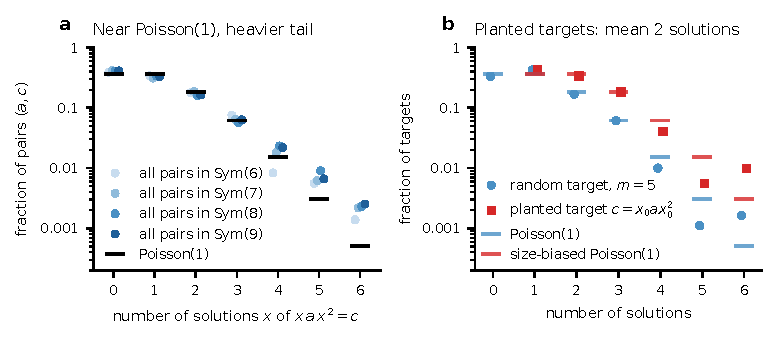
\includegraphics[width=\textwidth]{fig_statistics}
\caption{Statistics of the solution count of $x\,a\,x^{2}=c$. (a) Fraction of pairs $(a,c)\in\Sym(N)^{2}$ with exactly $k$ solutions, from exhaustive tables for $N=6,7,8,9$ ($N!^{2}$ pairs each), against the Poisson(1) law; the excess at $k\ge4$ comes from structured pairs such as $a=c=1$. (b) Wreath instances at $m=5$, all $3600$ pairs $(A,B)$ and all $3600$ targets each: random targets follow Poisson(1), planted targets $c=x_0ax_0^{2}$ follow the size-biased law $k\,e^{-1}/k!$ with mean $2$.}
\label{fig:stat}
\end{figure}

\begin{thm}[first moment]\label{thm:firstmoment}\label{prop:moment}
Fix $a\in\Sym(N)$ of cycle type $\alpha$ and a conjugacy class $\gamma$. Then
\[ \sum_{c\in\gamma}\#\{x:\ x\,a\,x^{2}=c\}\;=\;\#\{x:\ \ctype(a\,x^{3})=\gamma\}\;=\;\sum_{\nu}\rho_3(\nu)\,K(\gamma,\nu;\alpha), \]
the sum over the conjugacy classes $\nu$ of $\Sym(N)$,
where $K(\gamma,\nu;\alpha)=\#\{(z,w)\in\gamma\times\nu: zw=a\}=\frac{|\gamma||\nu|}{N!}\sum_{\chi}\frac{\chi(\gamma)\chi(\nu)\chi(\alpha)}{\chi(1)}$
and, if $\nu$ has $m_L$ cycles of length $L$,
\[ \rho_3(\nu)=\#\{x: x^{3}=y\}\quad(y\in\nu\text{ fixed})\quad=\ \prod_L\ \sum_{k}\frac{m_L!}{(m_L-3k)!\,k!\,6^{k}}\,(2L^{2})^{k}, \]
the inner sum over $0\le k\le m_L/3$, restricted to $3k=m_L$ when $3\mid L$.
\end{thm}
\begin{proof}
$xax^{2}=x(ax^{3})x^{-1}$, so $c=xax^{2}\in\gamma$ iff $ax^{3}\in\gamma$; summing over $c\in\gamma$ counts the $x$ with $\ctype(ax^{3})=\gamma$.
Group them by $y=x^{3}$: the number of cube roots of $y$ is a class function $\rho_3(\ctype y)$, and the number of $y\in\nu$ with $ay\in\gamma$
equals $\#\{(z,w)\in\gamma\times\nu: zw=a\}$ via $z=ay$, $w=y^{-1}$. For $\rho_3$: an $x$-cycle of length $m$ with $3\nmid m$ cubes to one
$m$-cycle, one with $3\mid m$ cubes to three $m/3$-cycles; so the $L$-cycles of $y$ are partitioned into singletons (only if $3\nmid L$; the root
on that cycle is the unique power $y_0^{t}$, $3t\equiv1$) and unordered triples merged into a $3L$-cycle of $x$ ($2L^{2}$ interleavings each).
\end{proof}
The right-hand side depends only on $\alpha$ and $\gamma$. Its evaluation is polynomial in the number $p(N)=e^{\Theta(\sqrt N)}$ of classes once the character table of $\Sym(N)$ is available, but we know no algorithm polynomial in $N$; the identity is a statement about averages, not an algorithm. It was checked against the exhaustive tables on all $1813$ pairs of classes $(\alpha,\gamma)$ for $3\le N\le9$ (the first equality alone on the $121$, $225$ and $484$ blocks at $N=6,7,8$). It gives the average of the solution count over a block of pairs in closed form; inside a block the counts are approximately Poisson with that mean, and nothing in the identity constrains an individual pair. The identity reduces to two classical counts -- the fibres of the cube map on $\Sym(N)$ \cite{chowla1951,moser1955,pavlov1981,chernoff1994} and the structure constants of the class algebra \cite{goupil1990,bedard1992} -- and we have not found it stated in the literature.

\subsection{No word invariant decides solvability}

Since conjugacy is decided by a cycle type, one may ask whether solvability of $\Pthree$ is decided by cycle types of short words in $a$ and $c$, or by the orbit structure of $\langle a,c\rangle$.

\begin{thm}[no word invariant decides $\Pthree$]\label{thm:psl}
Let $a=(0\,1\,2\,3\,4\,5\,6)\in\Sym(7)$, $c_1=[0,4,5,1,3,6,2]$ and $c_2=[0,2,5,6,3,1,4]$ (image tuples). Then $x\,a\,x^{2}=c_1$ has no solution
and $x\,a\,x^{2}=c_2$ has exactly one. There is an isomorphism $\varphi:\langle a,c_1\rangle\to\langle a,c_2\rangle$ (both isomorphic to
$\mathrm{PSL}(2,7)$, of order $168$, transitive on $[7]$) with $\varphi(a)=a$, $\varphi(c_1)=c_2$ and $\ctype(\varphi(g))=\ctype(g)$ for every $g$.
Consequently $\ctype\,w(a,c_1)=\ctype\,w(a,c_2)$ for \emph{every} word $w$ in $a^{\pm1},c^{\pm1}$, and the two pairs have the same orbit
structure, group order, isomorphism type and permutation character: no function of these data decides solvability or the number of solutions.
\end{thm}
\begin{proof}
Proof by finite certificate. Enumerate $G_1=\langle a,c_1\rangle$ by breadth-first search, recording for each $g$ one word $w_g$ with
$g=w_g(a,c_1)$, and put $\varphi(g)=w_g(a,c_2)$. Check $\varphi(gh)=\varphi(g)\varphi(h)$ for all $168^{2}$ pairs: this makes $\varphi$ a
homomorphism, and then every word evaluating to $g$ at $(a,c_1)$ evaluates to $\varphi(g)$ at $(a,c_2)$ (induction on the length), so
$\varphi$ does not depend on the chosen words. Check that $\varphi$ is injective, hence an isomorphism onto $G_2=\langle a,c_2\rangle$
($|G_2|=168$), and that $\ctype\varphi(g)=\ctype g$ for all $g$. Then $w(a,c_2)=\varphi(w(a,c_1))$ has the cycle type of $w(a,c_1)$ for
every word $w$; both groups are transitive; and the permutation characters satisfy $\pi_2\circ\varphi=\pi_1$, since the number of fixed
points is read off the cycle type. The solution counts are obtained by brute force over $\Sym(7)$. (Recorded in \texttt{counting\_track.py} and re-verified in \texttt{verify\_campaign.py}.)
\end{proof}
\begin{rem}
The two groups $G_1=\langle a,c_1\rangle$ and $G_2=\langle a,c_2\rangle$ are conjugate in $\Sym(7)$ (by odd permutations only), but
$\varphi$ is not induced by any element of $\Sym(7)$: composed with a conjugation it is the outer automorphism of $\mathrm{PSL}(2,7)\cong
\mathrm{GL}(3,2)$, which exchanges the actions on the points and on the lines of the Fano plane. The natural $G_1$-set $[7]$ and the same set with the action twisted by $\varphi$ therefore have the same permutation character without being isomorphic as $G_1$-sets: this is the classical Gassmann triple of degree $7$ \cite{perlis1977,sunada1985,kammeyer2024gassmann}. Gassmann equivalence is usually invoked to produce arithmetically equivalent number fields or isospectral manifolds;
here it shows that solvability of $x\,a\,x^{2}=c$ is not a function of any word-cycle-type invariant of the pair $(a,c)$.
\end{rem}
\begin{rem}
Smaller witnesses exist for shorter words: at $N=6$, $a=(0\,1\,2\,3\,4\,5)$, $c_1=(0\,5)(1\,3)$ has no solution and $c_2=(0\,5)(2\,4)$ has one, while the cycle types of all words of length at most four and the orbit structure coincide; a word of length seven separates them. At $N=7$ no word separates the pairs of Theorem~\ref{thm:psl}. In the exhaustive tables, the cycle types of words of length at most $L$ determine the solution count only when they are close to a complete invariant of the simultaneous-conjugacy class of $(a,c)$ (for $a$ a $7$-cycle, words of length $\le8$ separate $705$ of the $726$ pair classes and still do not decide).
\end{rem}
The tautological complete invariant -- the simultaneous-conjugacy class of the pair $(a,c)$ -- has at least $N!/|\Cent(a)|$ values, and every coarsening we tested fails.

\begin{rem}[the $N$-cycle family is rigid but not easier]
For $a$ an $N$-cycle, $\Cent(a)=\langle a\rangle$, so every solution of $\Pthree(a,c)$ with $c\notin\langle a\rangle$ moves $a$; the mechanisms of Theorem~\ref{thm:main} are polynomial-time here (order-$3$ solutions form at most $N$ candidates; for $c\in\langle a\rangle$ all solutions were found
affine for $N\le11$). Exhaustive tables for $N\le11$ give a solvable fraction between $0.597$ and $0.667$, the symmetry group of the solvable
set inside the affine normaliser of $\langle a\rangle$ is exactly $\langle a\rangle$ (the family is chiral: at $N=4$, $c=(1\,2\,3)$ has two solutions
and $c=(1\,3\,2)$ none), and none of the natural rotation invariants of $c$ decides solvability from $N=6$ on. Restricting $a$ to pairwise
distinct cycle lengths or to lengths coprime to $3$ changes neither the solvable fraction nor the solver cost.
\end{rem}

\section{Conjugacy by an element of prime order}\label{sec:hard}

\begin{defi}[\textsc{Order-3 Conjugacy}, $\Dzero$]\label{def:dzero}
\emph{Input:} $a,c\in\Sym(N)$. \emph{Question:} is there $x\in\Sym(N)$ with $x^{3}=1$ and $x\,a\,x^{-1}=c$?
\end{defi}
Since $x^{2}=x^{-1}$ when $x^{3}=1$, $\Dzero$ is the restriction of $\Pthree$ to solutions of order dividing $3$; equivalently, it asks whether the coset $g\Cent(a)$ of all conjugators of $a$ to $c$ contains an element of order dividing $3$.

\begin{thm}\label{thm:main}
$\Dzero$ is NP-complete. Hardness holds already when $a$ consists of $k$ disjoint cycles of one prime length $L\equiv2\pmod3$ (depending on the instance), when $c\in\Cent(a)$, and when the certificate is required to have cycle type $3^{N/3}$.
\end{thm}

\subsection{Conjugators between blockwise translations}\label{sec:block}

Fix a prime $L\ge5$ and $k\ge1$, put $N=kL$, and identify the block $B_i=\{iL,\ldots,iL+L-1\}$ with $\ZZ_L$ via $iL+z\mapsto z$. Let $a$ act on every block as $z\mapsto z+1$. For units $m_1,\ldots,m_k\in\ZZ_L^{\times}$ let $c=c(m)$ act on $B_i$ as $z\mapsto z+m_i$; thus $c|_{B_i}=a^{m_i}|_{B_i}$, $c\in\Cent(a)$, and every block is a cycle of $c$.

\begin{lem}[block lemma]\label{lem:block}
$x\,a\,x^{-1}=c(m)$ if and only if there are $\sigma\in\Sym(k)$ and $t_1,\ldots,t_k\in\ZZ_L$ such that $x$ maps $B_i$ onto $B_{\sigma(i)}$ by the affine map $x(z)=m_{\sigma(i)}z+t_i$.
\end{lem}
\begin{proof}
A conjugator maps cycles of $a$ onto cycles of $c$ of the same length, i.e.\ blocks onto blocks, and satisfies $x(a(p))=c(x(p))$, which on $B_i$ with $x(B_i)=B_{\sigma(i)}$ reads $x(z+1)=x(z)+m_{\sigma(i)}$. Its solutions are exactly the affine maps displayed, and each such family conjugates $a$ to $c(m)$.
\end{proof}

\begin{lem}[affine criterion]\label{lem:affine}
$\Dzero(a,c(m))$ has a solution iff there is $\sigma\in\Sym(k)$ with $\sigma^{3}=1$ such that (i) $m_im_jm_l\equiv1\pmod L$ for every $3$-cycle $(i\,j\,l)$ of $\sigma$ and (ii) $m_i^{3}\equiv1\pmod L$ for every fixed point $i$ of $\sigma$. If all $m_i\neq1$ and $L\equiv2\pmod3$, (ii) is never satisfiable and every solution has cycle type $3^{N/3}$.
\end{lem}
\begin{proof}
By Lemma~\ref{lem:block}, $x$ permutes the blocks via $\sigma$, so $x^{3}=1$ forces $\sigma^{3}=1$. On a $3$-cycle $i\mapsto j\mapsto l\mapsto i$, $x^{3}|_{B_i}$ is a composite of three affine maps with slopes $m_j,m_l,m_i$; it is the identity iff the slope product is $1$ and the translation part vanishes, and the translation part is an affine expression in $(t_i,t_j,t_l)$ in which $t_l$ has coefficient $1$, so it can always be made zero. On a fixed block, $x|_{B_i}(z)=m_iz+t_i$ and $x^{3}(z)=m_i^{3}z+(1+m_i+m_i^{2})t_i$; if $m_i=1$ take $t_i=0$ (as $L\neq3$); if $m_i\neq1$ and $m_i^{3}=1$ then $1+m_i+m_i^{2}=0$ and any $t_i$ works; if $m_i^{3}\neq1$ nothing works. For $L\equiv2\pmod3$, $\ZZ_L^{\times}$ has order $L-1\not\equiv0\pmod3$ and no element of order $3$, so $m_i^{3}=1$ forces $m_i=1$.
\end{proof}
Writing $m_i=g^{e_i}$ for a generator $g$ of $\ZZ_L^{\times}$, condition (i) reads $e_i+e_j+e_l\equiv0\pmod{L-1}$: on this family $\Dzero$ is a zero-sum triple-partition problem in $\ZZ_{L-1}$. (Lemma~\ref{lem:affine} was verified against exhaustive enumeration of all $L^{k}k!$ conjugators on $160$ random instances with $(L,k)\in\{(5,3),(7,3),(5,4),(11,3)\}$, and on $2832$ further instances up to $N=33$.)

\begin{figure}[htbp]\centering
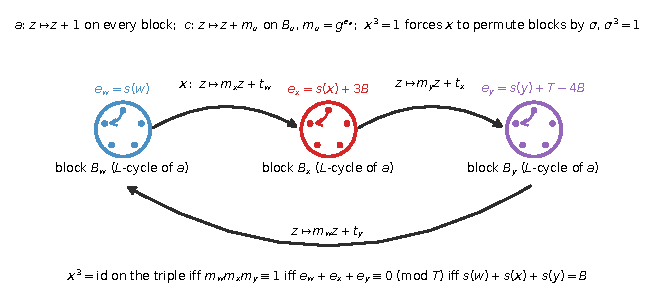
\includegraphics[width=\textwidth]{fig_reduction}
\caption{The reduction of Theorem~\ref{thm:main}. Each element $u\in W\cup X\cup Y$ of the N3DM instance becomes a block $B_u\cong\ZZ_L$ on which $a$ is the translation by $1$ and $c$ the translation by $m_u=g^{e_u}$. A conjugator of order three permutes the blocks by $\sigma$ with $\sigma^{3}=1$ and acts on each block by an affine map $z\mapsto m_{\sigma(u)}z+t_u$ (Lemma~\ref{lem:block}); a $\sigma$-triple has $x^{3}=1$ iff the product of its three slopes is $1$, i.e.\ iff its exponents sum to $0$ modulo $T=L-1$, which the choice of exponents makes equivalent to the matching condition $s(w)+s(x)+s(y)=B$ (Lemma~\ref{lem:affine} and the case analysis in the proof).}
\label{fig:red}
\end{figure}

\subsection{The reduction}

\textsc{Numerical 3-Dimensional Matching} (N3DM): given disjoint sets $W,X,Y$ of $q$ elements, sizes $s(u)\in\{1,\ldots,B\}$ and the bound $B$, decide whether $W\cup X\cup Y$ can be partitioned into $q$ triples, each with one element of $W$, of $X$ and of $Y$, with $s(w)+s(x)+s(y)=B$ in every triple. N3DM is strongly NP-complete \cite[SP16]{garey1979}, so $B$ may be assumed given in unary.

\begin{proof}[Proof of Theorem~\ref{thm:main}]
Membership in NP is clear. Given an N3DM instance (Figure~\ref{fig:red}), put $M=3B$ and let $L$ be the least prime with $L\equiv2\pmod3$ and $T:=L-1>12B$. By the prime number theorem
for arithmetic progressions, $L=O(B)$ with an absolute implied constant, which need not be known: $L$ is found by testing the candidates
$12B+2,12B+3,\dots$ by trial division, each test taking time polynomial in $B$. (The variant of Theorem~\ref{thm:conjp} with $L$ a power
of two avoids primes altogether.) Put $k=3q$, $N=kL$, and define exponents in $\ZZ_T$
\begin{align*}
 e_w&=s(w) &(w\in W),\\
 e_x&=s(x)+M &(x\in X),\\
 e_y&=s(y)+T-M-B &(y\in Y),
\end{align*}
$m_u=g^{e_u}$, and $(a,c)=(a,c(m))$ with one block per element $u$. The construction is polynomial in $q+B$.

No exponent is $0$: $e_w\in[1,B]$, $e_x\in[M+1,M+B]$ with $M+B<T$, and $e_y\in[T-M-B+1,T-M]$. Hence all $m_u\neq1$ and, by Lemma~\ref{lem:affine}, a solution of $\Dzero(a,c)$ is a partition of the blocks into triples with exponent sum $\equiv0\pmod T$, of cycle type $3^{N/3}$.

Let a triple contain $\alpha,\beta,\gamma$ elements of $W,X,Y$ ($\alpha+\beta+\gamma=3$) with size sum $S\in[3,3B]$. Its exponent sum is $S+\beta M+\gamma(T-M-B)\equiv S+(\beta-\gamma)M-\gamma B\pmod T$. With $M=3B$ and $T>12B$:
$(\alpha,\beta,\gamma)=(1,1,1)$ gives $S-B\in[3-B,2B]$, which is $\equiv0$ iff $S=B$;
$\gamma=0$ gives $S+\beta M\in[3,12B]$, never $\equiv0$;
$\gamma=1,\beta=0$ gives $S-M-B\in[3-4B,-B]$ and $\gamma=1,\beta=2$ gives $S+M-B\in[2B+3,5B]$, never $\equiv0$;
$\gamma=2$ gives $S+(\beta-2)M-2B\in[3-8B,-2B]$, never $\equiv0$;
$\gamma=3$ gives $S-3M-3B\in[3-12B,-9B]$, never $\equiv0$.
So the admissible triples are exactly the matching triples, and $\Dzero(a,c)$ is solvable iff the N3DM instance is. Every certificate has cycle type $3^{N/3}$ and $c\in\Cent(a)$.
\end{proof}
The case analysis was verified exhaustively for $B\le40$ and three values of $T$, the reduction against brute force on $180$ random N3DM instances ($q\le3$), and, at $q=1$, against exhaustive enumeration of all conjugators on eleven instances with $N$ up to $267$.

\subsection{Conjugacy by an element of prescribed order}\label{sec:conjn}
For an integer $n\ge1$ let $\Conj{n}$ be the problem: given $a,c\in\Sym(N)$, is there $x\in\Sym(N)$ with $x^{n}=1$ and $xax^{-1}=c$?
Since $x=1$ is a solution iff $a=c$, requiring order exactly $n$ or order dividing $n$ gives polynomially equivalent problems (the exact-order
variant for $n=2$ is treated at the end of the proof of Theorem~\ref{thm:conjn}); for $n=3$ this is the problem of Definition~\ref{def:dzero}.
This subsection classifies $\Conj{n}$ over all $n$: it is polynomial for $n\in\{1,2\}$ and NP-complete for every $n\ge3$.

\paragraph{The affine criterion for $x^{n}=1$}
We use the blockwise family of Section~\ref{sec:block} with an arbitrary modulus $L\ge3$ (not necessarily prime): $a$ acts on each of $k$
blocks $B_i\cong\ZZ_L$ as $z\mapsto z+1$ and $c=c(m)$ as $z\mapsto z+m_i$ with $m_i\in\ZZ_L^{\times}$; thus $c\in\Cent(a)$ and $c$ has the
same cycle type as $a$. Lemma~\ref{lem:block} and its proof hold verbatim: the conjugators of $a$ to $c$ are the maps sending $B_i$ onto
$B_{\sigma(i)}$ by $z\mapsto m_{\sigma(i)}z+t_i$, $\sigma\in\Sym(k)$, $t\in\ZZ_L^{k}$.

\begin{lem}[affine criterion for $x^{n}=1$]\label{lem:affinen}\label{lem:affinep}
Let $n\ge1$, $L\ge3$ and $a,c(m)$ be as above. $\Conj{n}(a,c(m))$ has a solution iff there is $\sigma\in\Sym(k)$ with
$\sigma^{n}=1$ such that for every cycle $C$ of $\sigma$, writing $R_C=\prod_{i\in C}m_i$,
\[ R_C^{\,n/|C|}\equiv1\pmod L. \]
When the condition holds, $x$ defined by $x(z)=m_{\sigma(i)}z$ on $B_i$ (all translations zero) is a solution; moreover
$x^{d}\neq1$ for every $d<n$ that is not a multiple of the order of $\sigma$.
\end{lem}
\begin{proof}
Let $x$ be a conjugator with block permutation $\sigma$ and translations $t$ (block lemma). Then $x^{j}$ maps $B_i$ onto
$B_{\sigma^{j}(i)}$, so $x^{n}=1$ forces $\sigma^{n}=1$; thus every cycle $C=(i_1\,i_2\cdots i_\ell)$ of $\sigma$ has length
$\ell\mid n$. On $B_{i_1}$, $x^{\ell}$ is the composite of the $\ell$ affine maps $z\mapsto m_{i_2}z+t_{i_1}$,
$z\mapsto m_{i_3}z+t_{i_2}$, \dots, $z\mapsto m_{i_1}z+t_{i_\ell}$, hence an affine map $z\mapsto R_Cz+\tau_C$ with
$R_C=\prod_{i\in C}m_i$; and $x^{n}|_{B_{i_1}}=(x^{\ell}|_{B_{i_1}})^{n/\ell}$ is $z\mapsto R_C^{n/\ell}z+(1+R_C+\dots+R_C^{n/\ell-1})\tau_C$.
An affine map $z\mapsto\alpha z+\beta$ of $\ZZ_L$ ($L\ge3$) is the identity iff $\beta=0$ (take $z=0$) and $\alpha=1$ (take $z=1$).
So $x^{n}=1$ implies $R_C^{n/\ell}\equiv1$ for every cycle: the condition is necessary.
Conversely, if $\sigma^{n}=1$ and $R_C^{n/|C|}\equiv1$ for all cycles, take $t\equiv0$. By the block lemma $x$ conjugates $a$ to $c(m)$;
on each block of a cycle $C$ of length $\ell$, $x^{\ell}$ is the linear map $z\mapsto R_Cz$ (the product is taken in the cyclic order
starting at that block, but all cyclic rotations of a product of elements of the abelian group $\ZZ_L^{*}$ coincide), so
$x^{n}|_{B_i}=(z\mapsto R_C^{n/\ell}z)=\mathrm{id}$ on every block, i.e.\ $x^{n}=1$. Finally $x^{d}$ moves $B_i$ to
$B_{\sigma^{d}(i)}\ne B_i$ whenever $\sigma^{d}\ne1$, so $x^{d}\ne1$ for such $d$.
\end{proof}

For $n=p$ prime the criterion reads: the product of the slopes over every $p$-cycle of $\sigma$ is $1$ and $m_i^{p}=1$ on every fixed
point; if $\ZZ_L^{\times}$ has no element of order $p$ and $m_i\neq1$ for all $i$, every solution has cycle type $p^{N/p}$.

\paragraph{Hardness for every $n\ge3$}
\emph{Numerical $n$-Dimensional Matching} ($\mathrm{N}n\mathrm{DM}$): given $n$ disjoint classes $C_1,\dots,C_n$ of $q$ elements each, sizes
$s(u)\in\{1,\dots,B'\}$ and the target $B'$ (in unary), decide whether $\bigcup C_j$ splits into $q$ $n$-tuples, one element per class, each of
size-sum $B'$. For $n=3$ this is N3DM, strongly NP-complete \cite[SP16]{garey1979}. For $n>3$, padding an N3DM instance with $n-3$ classes of
$q$ elements of size $1$ and target $B'=B+n-3$ gives an equivalent instance, so $\mathrm{N}n\mathrm{DM}$ is strongly NP-complete for every fixed $n\ge3$.
The encoding of a matching instance into slopes uses the integers
\begin{align*} M&=nB'+1,& w_j&=(n+1)^{j-1}\quad(1\le j\le n-1),\\ W&=\sum_{j<n}w_j=\frac{(n+1)^{n-1}-1}{n},& T_0&=M(n+1)^{n-1}, \end{align*}
and, for an integer $T\ge T_0$, the exponents $e_u=s(u)+Mw_j$ for $u\in C_j$, $j<n$, and $e_u=s(u)-MW-B'$ for $u\in C_n$.

\begin{lem}[encoding lemma, composite $n$]\label{lem:encn}
Let $n\ge3$, $T\ge T_0$, and let $S\subseteq\bigcup_jC_j$ with $|S|=\ell$, $\ell\mid n$. Then
\[ \frac{n}{\ell}\sum_{u\in S}e_u\equiv0\pmod T \iff \ell=n,\ \ |S\cap C_j|=1\ \text{for all } j,\ \ \sum_{u\in S}s(u)=B'. \]
\end{lem}
\begin{proof}
Put $\beta_j=|S\cap C_j|$, $\Sigma=\sum_{u\in S}s(u)\in[\ell,\ell B']$ and $D=\sum_{j<n}w_j(\beta_j-\beta_n)\in\ZZ$. Summing the
definitions gives the integer identity
\[ \sum_{u\in S}e_u=\Sigma-\beta_nB'+MD. \tag{1} \]
\emph{Size bound.} Every $e_u$ satisfies $|e_u|\le E:=MW+B'$ (for $j<n$: $0<e_u\le B'+Mw_{n-1}\le E$; for $j=n$:
$e_u\in[1-MW-B',\,-MW]$). Now $nE=M\bigl((n+1)^{n-1}-1\bigr)+nB'=T_0-M+nB'=T_0-1<T$, hence
\[ \Bigl|\sum_{u\in S}e_u\Bigr|\le\ell E<\frac{\ell}{n}\,T\le\frac{T}{\gcd(n/\ell,\,T)}. \]
Since $\frac n\ell\,y\equiv0\pmod T$ iff $y\equiv0\pmod{T/\gcd(n/\ell,T)}$, the left-hand side of the lemma holds iff
$\sum_{u\in S}e_u=0$ as an integer.
\emph{(a) $D=0$ iff all $\beta_j$ are equal.} Put $d_j=\beta_j-\beta_n\in[-\ell,\ell]\subseteq[-n,n]$. If some $d_j\ne0$ and $j_0$ is the
least such index, $D\equiv(n+1)^{j_0-1}d_{j_0}\pmod{(n+1)^{j_0}}$, so $D=0$ would force $(n+1)\mid d_{j_0}$, impossible for
$0<|d_{j_0}|\le n$. If all $\beta_j$ equal $\beta$ then $n\beta=\ell\le n$, so $\beta=1$ and $\ell=n$ ($S\ne\emptyset$).
\emph{(b)} If $D=0$ then $\beta_n=1$, $\ell=n$, and (1) reads $\Sigma-B'$, which vanishes iff $\Sigma=B'$.
\emph{(c)} If $D\ne0$ then $|MD|\ge M>M-1=nB'\ge|\Sigma-\beta_nB'|$ (as $\Sigma\le\ell B'\le nB'$ and $\beta_nB'\le nB'$), so (1) is
nonzero. Together: the integer sum vanishes iff $\ell=n$, one element per class, and $\Sigma=B'$.
\end{proof}

\begin{thm}[conjugacy by an element of order $n$]\label{thm:conjn}\label{thm:conjp}
For every integer $n\ge3$, $\Conj{n}$ is NP-complete. Hardness holds already when $a$ consists of $k$ disjoint cycles of one length $L$ (depending on the instance), with $L$ prime or a power of two, when $c\in\Cent(a)$, and when the certificate is required to have cycle type
$n^{N/n}$, i.e.\ order exactly $n$. Consequently, unless $\mathrm P=\mathrm{NP}$, $\Conj{n}$ is polynomial iff $n\in\{1,2\}$,
and the same holds for the variant asking for a conjugator of order exactly $n$.
\end{thm}
\begin{proof}
Membership in NP is clear. Fix $n\ge3$ and let an $\mathrm{N}n\mathrm{DM}$ instance $(C_1,\dots,C_n;s;B')$ be given. With $M,w_j,W,T_0$
and $e_u$ as in Lemma~\ref{lem:encn}, let $L$ be the least prime with $T:=L-1\ge T_0$ (by Bertrand's postulate $L\le2T_0+2$, found by trial
division in time polynomial in $T_0$) and $g$ a primitive root mod $L$ (found by exhaustive search, $L$ being polynomial in the input);
alternatively $L=2^{r}$ with $T=2^{r-2}\ge T_0$ and $g=5$, of order $T$ in $\ZZ_L^{\times}$. Put $m_u=g^{e_u}$, $k=nq$, $N=kL$, and let
$(a,c)=(a,c(m))$ be the blockwise instance; $N=\Theta(qB'(n+1)^{n-1})$ is polynomial in $q+B'$ for fixed $n$. As $g$ has order $T$,
for every set $S$ of blocks with $|S|=\ell$, $R_S:=\prod_{u\in S}m_u=g^{\sum_Se_u}$ satisfies
$R_S^{n/\ell}=1$ iff $\frac n\ell\sum_{u\in S}e_u\equiv0\pmod T$.

By Lemma~\ref{lem:affinen}, $\Conj{n}(a,c)$ has a solution iff the blocks can be partitioned into the cycles of some
$\sigma$ with $\sigma^{n}=1$ such that each cycle $S$ (of length $\ell\mid n$) satisfies $R_S^{n/\ell}=1$; by Lemma~\ref{lem:encn} a set
$S$ with $|S|\mid n$ satisfies this iff it is a matching $n$-tuple (one element per class, size-sum $B'$). Hence
$\Conj{n}(a,c)$ is solvable iff the blocks can be partitioned into matching $n$-tuples, i.e.\ iff the $\mathrm{N}n\mathrm{DM}$
instance is a yes-instance. In that case every solution $x$ has block permutation $\sigma$ consisting of $n$-cycles only, so every
orbit of $x$ has size exactly $n$ ($x^{d}$ moves every block for $0<d<n$): the certificates have cycle type $n^{N/n}$, and
requiring order exactly $n$ changes nothing. Since $\mathrm{N}n\mathrm{DM}$ is strongly NP-complete for fixed $n\ge3$, so is
$\Conj{n}$ (NP-hard, in NP). With $\Conj{1}$ trivial and $\Conj{2}\in\mathrm P$ (Theorem~\ref{thm:conj2}), the classification
follows; for the exact-order variant with $n=2$, if $a\ne c$ every solution of $x^{2}=1$ is an involution, and if $a=c$ the question is
whether $\Cent(a)$ contains an involution, which holds iff $a$ has a cycle of even length or two cycles of the same length (read off the
cycle type).
\end{proof}

\begin{rem}
For $n=3$ this recovers Theorem~\ref{thm:main} with different constants and adds the variant with cycles of $2$-power length, which needs no
theorem on primes. The reduction is polynomial for each fixed $n$ but exponential in $n$ ($N=\Theta(qB'(n+1)^{n-1})$); $\Conj{n}$ with $n$
part of the input is NP-complete since it contains $\Conj{3}$, but whether it admits a reduction polynomial in $n$ is open. The ``adjoin a
gadget of order $m$'' route from $\Conj{p}$ to $\Conj{pm}$ by disjoint union does not work in general: the conjugators of $(0\,1\,2\,3\,4)$ to
its square all have order $4$, and those of a $7$-cycle to its cube all have order $6$, so $\Conj{pm}(a,c)$ and $\Conj{p}(a,c)$ differ.
\end{rem}

\paragraph{Conjugacy by an involution is polynomial}
Let $G=\langle a,c\rangle$. For a word $w$ in two letters write $w^{\tau}$ for the word with the letters exchanged. A \emph{plain isomorphism}
between $G$-orbits $O,O'$ is a bijection commuting with $a$ and $c$; a \emph{twisted isomorphism} is a bijection $\varphi$ with $\varphi a=c\varphi$
and $\varphi c=a\varphi$ on $O$.

\begin{lem}\label{lem:inv1}
Let $x^{2}=1$ and $xax^{-1}=c$. Then $xcx^{-1}=a$, $x$ normalises $G$ and permutes its orbits, $x|_O$ is a twisted isomorphism $O\to x(O)$ for
every orbit $O$, and $x$ is determined on $O$ by the image of one point: $x(w(a,c)j_0)=w(c,a)\,x(j_0)$.
\end{lem}
\begin{proof}
$xcx^{-1}=x^{2}ax^{-2}=a$. Hence $xgx^{-1}=g^{\tau}\in G$ for $g\in G$, and $x(gj_0)=g^{\tau}x(j_0)$; $G$ is transitive on $O$.
\end{proof}

\begin{lem}\label{lem:inv2}
Let $O$ be a $G$-orbit and $j_0\in O$. (a) For each $v$ there is at most one twisted isomorphism $O\to Gv$ with $j_0\mapsto v$, and its existence is
decided in $O(|O|)$ time by closing $x(au)=c\,x(u)$, $x(cu)=a\,x(u)$ from $x(j_0)=v$ and checking consistency and injectivity.
(b) A twisted automorphism $x$ of $O$ satisfies $x^{2}=1$ iff $x^{2}(j_0)=j_0$. (c) If $O\ne O'$ and $\varphi:O\to O'$ is a twisted isomorphism,
then $\varphi\cup\varphi^{-1}$ is an involution of $O\cup O'$ conjugating $a$ to $c$ there.
\end{lem}
\begin{proof}
(a) A twisted isomorphism $\varphi$ with $\varphi(j_0)=v$ satisfies $\varphi(w(a,c)\,j_0)=w(c,a)\,v$ for every word $w$ (induction on the
length of $w$), and $G$ is transitive on $O$, so $\varphi$ is unique. To decide its existence, propagate $\varphi(au)=c\,\varphi(u)$ and
$\varphi(cu)=a\,\varphi(u)$ from $\varphi(j_0)=v$ along the Schreier graph of $O$; every point of $O$ carries one $a$-edge and one $c$-edge,
so $2|O|$ equations are examined. If no conflict occurs the resulting map satisfies $\varphi a=c\varphi$ and $\varphi c=a\varphi$ on $O$,
its image is a non-empty $\langle a,c\rangle$-invariant subset of the orbit $Gv$, hence all of $Gv$, and it is a bijection iff it is
injective, which is checked in $O(|O|)$ time. (b) $x^{2}a=xcx=ax^{2}$ and likewise $x^{2}c=cx^{2}$, so $x^{2}$ is a plain automorphism of the
transitive $G$-set $O$; a plain automorphism fixing a point is the identity. (c) On $O$, $\psi=\varphi$ gives $\psi a=c\psi$; on $O'$,
$\psi=\varphi^{-1}$ and $\varphi c=a\varphi$ give $\varphi^{-1}a=c\varphi^{-1}$, i.e.\ $\psi a=c\psi$; and $\psi^{2}=1$.
\end{proof}

\begin{thm}\label{thm:conj2}
Partition the $G$-orbits into plain-isomorphism classes $\mathcal C_1,\dots,\mathcal C_s$; for a class $\mathcal C$ let $\mathcal C^{\tau}$ be the
class of orbits twisted-isomorphic to the orbits of $\mathcal C$, if any. Then $\Conj{2}(a,c)$ is a yes-instance iff for every class
$\mathcal C$: (1) $\mathcal C^{\tau}$ exists and $|\mathcal C^{\tau}|=|\mathcal C|$; and (2) if $\mathcal C^{\tau}=\mathcal C$ and $|\mathcal C|$ is odd,
one (equivalently every) orbit of $\mathcal C$ admits an involutive twisted automorphism, i.e.\ a twisted isomorphism $x\colon O\to O$ with $x^{2}=1$. The conditions are decidable, and a certificate
constructed, in $O(N^{3})$ time. In particular $\Conj{2}\in\mathrm P$.
\end{thm}
\begin{proof}
Necessity: by Lemma~\ref{lem:inv1} an involutive solution induces an involution on the set of orbits mapping $\mathcal C$ onto $\mathcal C^{\tau}$,
which gives (1); if $\mathcal C^{\tau}=\mathcal C$ has odd size, some orbit of $\mathcal C$ is fixed and $x$ restricts to an involutive twisted
automorphism of it, which transfers to every orbit of the class by conjugation with a plain isomorphism. Sufficiency: pair the orbits of
$\mathcal C$ with those of $\mathcal C^{\tau}$ (arbitrarily when $\mathcal C^{\tau}\ne\mathcal C$, among themselves when $\mathcal C^{\tau}=\mathcal C$),
use Lemma~\ref{lem:inv2}(c) on each pair and the involutive twisted automorphism of (2) on a leftover orbit; the pieces live on disjoint orbits
and their union satisfies $x^{2}=1$, $xa=cx$. Complexity: orbits in $O(N)$; each isomorphism test tries at most $|O'|$ images of $j_0$, each in
$O(|O|)$ time, so $O(N^{2})$ per pair of orbits and $O(N^{3})$ overall.
\end{proof}
\begin{rem}
For $c=a^{-1}$ the question is whether $a$ is \emph{strongly real}, which in $\Sym(N)$ always holds \cite{tiep2005real}; for general $c$
the problem of deciding whether some involution conjugates $a$ to $c$ does not seem to have been considered, and Theorem~\ref{thm:conj2}
settles it. The criterion was checked against brute force over all involutions of $\Sym(N)$ on $1520$ pairs with $N\le7$
(\texttt{verify\_campaign.py}) and, independently, on all $873$ pairs $(a,c)$ with $N\le6$, one $a$ per cycle type and every $c$ conjugate
to $a$, plus $300$ random pairs at $N=7$ (\texttt{audit\_checks.py}), and on $409\,113$ pairs with $N\le9$ (\texttt{conj\_p\_track.py}):
no discrepancy. Lemma~\ref{lem:affinen} was checked against exhaustive enumeration of all $L^{k}k!$ conjugators on $392$ instances with
$L\in\{4,5,6,7,8,9\}$ and $n\in\{2,3,4,6,8,9,12\}$ (\texttt{verify\_round2.py}) and on the instances of \texttt{conj\_composite\_track.py};
the reduction of Theorem~\ref{thm:conjn} was run against brute-force matching for $n\in\{3,4,6,9\}$ on $80$ instances, with explicit
certificates built and checked for $n\in\{3,4,6\}$.
\end{rem}

\begin{cor}\label{cor:classification}
Unless $\mathrm P=\mathrm{NP}$, the problem ``the coset of conjugators of $a$ to $c$ contains an element of order $n$'' (or of order dividing $n$)
is polynomial exactly for $n\in\{1,2\}$. The dichotomy has a structural reason: for $n=2$ the solution normalises $\langle a,c\rangle$ and is
determined by one image per orbit; for $n\ge3$, $xcx^{-1}=x^{2}ax^{-2}$ is a new permutation and the freedom it leaves is enough to encode
$\mathrm{N}n\mathrm{DM}$.
\end{cor}

\subsection{Consequences for \texorpdfstring{$\Pthree$}{P3}}

For a partition $\lambda$ of $N$ let $\Pthree^{\lambda}$ be $\Pthree$ restricted to solutions with $\ctype(x)=\lambda$.
\begin{cor}\label{cor:lambda}
$\Pthree^{\lambda}$ is NP-complete for $\lambda=3^{N/3}$; it is polynomial when all parts of $\lambda$ are at most $2$ (then $x^{2}=1$, so $x=ca^{-1}$ and one checks $\ctype(ca^{-1})=\lambda$), and in time $N^{O(s)}$ when the parts of $\lambda$ larger than $1$ sum to at most $s$ (then $|\supp x|\le s$, and the at most $N^{s}$ candidates are checked directly); by Lemma~\ref{lem:support} the bound $N^{O(s)}$ also holds for every $\lambda$ when $|\supp a|\le s$.
\end{cor}
\begin{cor}\label{cor:noenum}
Unless $\mathrm P=\mathrm{NP}$, no algorithm for $\Pthree$ can enumerate the $e^{O(\sqrt N)}$ cycle types of the unknown and decide each $\Pthree^{\lambda}$ in polynomial time; the cycle-type enumeration route does not yield a subexponential algorithm for $\Pthree$.
\end{cor}
Numerically, at $N=7,8,9$ exactly the types with all parts at most $2$ are decided by the cycle types of words of length at most four for every $a$ (and, for $N\le9$ only, the types of order three); every $\lambda$ with a part $\ge4$, or two parts $\ge3$, fails them already at $N=7$, and the decisions that appear for longer words occur only where those words are nearly a complete invariant of the pair class.

\begin{rem}[what Theorem~\ref{thm:main} does not prove]\label{rem:notproved}
On the hard family $\Pthree$ itself is trivially solvable: $x$ acting on every block as the translation by $(m_i-1)/3$ commutes with $a$ and satisfies $xax^{2}=ax^{3}=c$ (Lemma~\ref{lem:cent}). So the hardness of $\Dzero$ does not transfer to $\Pthree$ through this family, and ``rigid'' instances -- solvable pairs all of whose solutions have order exactly three -- are rare and become rarer: in exhaustive
censuses they are $7.1\%$, $6.2\%$, $3.3\%$ and $1.1\%$ of the solvable pairs for $N=5,6,7,8$, and $78\%$ of them have a unique solution at
$N=8$ (\texttt{audit\_checks.py}, \texttt{rigid\_census2}). Any hardness proof for $\Pthree$ must use solutions that move the constant, $xax^{-1}\neq a$.
\end{rem}

\begin{lem}[$\Dzero$ is a system of two $\Pthree$ equations]\label{lem:twoeq}
$\{x: x\,a\,x^{2}=c\ \text{and}\ x\,a^{2}x^{2}=c^{2}\}=\{x: x^{3}=1\ \text{and}\ xax^{-1}=c\}$.
\end{lem}
\begin{proof}
Write $b=xax^{-1}$ and $t=x^{3}$, so $xax^{2}=bt$ and $xa^{2}x^{2}=b^{2}t$. The first equation gives $b=ct^{-1}$; the second then reads
$ct^{-1}ct^{-1}=c^{2}t^{-1}$, i.e.\ $t^{-1}c=c$, so $t=1$ and $b=c$. The converse is immediate.
\end{proof}
\begin{rem}\label{rem:padding}
Hence the NP-completeness of Theorem~\ref{thm:main} is already attained by a \emph{system of two} equations of the shape $\Pthree$ with a common
unknown; the complexity of $\Pthree$ is exactly the question whether one equation can simulate the pair $(a,c),(a^{2},c^{2})$. Disjoint
padding cannot do it: if $a'=a\sqcup a_0$, $c'=c\sqcup c_0$ on $\Omega\sqcup\Omega_0$ then solutions of the two parts glue, and on the hard
family $\Pthree(a,c)$ is always solvable by the commuting cube root. Layered paddings on $\Omega\times\ZZ_M$ with $M\in\{2,3\}$ layers are
inert for the same reason (a blockwise-commuting layered solution exists whenever $L\nmid 2^{\ell}-(-1)^{\ell}$ for the layer-cycle lengths $\ell$).
\end{rem}

The only layered padding for which the small negative instances were solution-free is the four-layer construction below; it fails as well, and the first-moment identity explains why the zeros were accidental.

\begin{prop}[layered paddings do not reduce $\Dzero$ to $\Pthree$]\label{prop:fourlayer}
Let $a$ be a product of $k\ge1$ disjoint $5$-cycles on $\Omega$ (blocks $B_1,\dots,B_k\cong\ZZ_5$, $a$ the translation by $1$),
let $c=a^{-1}$ on $B_1$ and $c=a$ on $B_2,\dots,B_k$, and let $(a',c')$ be the four-layer padding on $\Omega\times\ZZ_4$,
\[
a'(j,r)=(a^{e_r}j,\;r+1),\qquad c'(j,r)=(c^{e_r}j,\;r+1),\qquad e=(1,2,3,3).
\]
Then $\Dzero(a,c)$ has no solution, whereas $x\,a'\,x^{2}=c'$ has at least $10$ solutions in $\Sym(\Omega\times\ZZ_4)$.
The same holds for every exponent vector $e\in\{1,2,3,4\}^{4}$ with $\sum_r e_r\not\equiv0$ and $\langle v,e\rangle\not\equiv0\pmod 5$,
$v=(1,2,4,3)$ (the $160$ vectors for which the blockwise-power ansatz of the padding is singular with the right-hand side outside its image).
In particular the padded instance $(a',c')$ is a YES instance of $\Pthree$ for a NO instance of $\Dzero$, for every $k$.
\end{prop}

\begin{proof}
\emph{$\Dzero(a,c)$ is NO.} By the block lemma (Lemma~\ref{lem:block}) a conjugator permutes the blocks by some $\sigma$ and acts on
$B_i$ by $z\mapsto m_{\sigma(i)}z+t_i$ with $m_1=4=-1$ and $m_i=1$ for $i\ge2$. By the affine criterion (Lemma~\ref{lem:affine}) an
order-$3$ conjugator needs $m_im_jm_l\equiv1$ on every $3$-cycle of $\sigma$ and $m_i^{3}\equiv1$ on every fixed block; the block $B_1$
lies either on a $3$-cycle, where the product is $(-1)\cdot1\cdot1=-1\not\equiv1$, or is fixed, where $(-1)^{3}=-1\not\equiv1\pmod5$.
(For $k=1$ this is the statement that every conjugator of a $5$-cycle to its inverse is a reflection $z\mapsto -z+t$, of order $\le2$.)

\emph{$\Pthree(a',c')$ is YES.} Both $a'$ and $c'$ preserve every set $B_i\times\ZZ_4$, so a disjoint union of solutions on the
$B_i\times\ZZ_4$ is a solution on $\Omega\times\ZZ_4$. On $B_i\times\ZZ_4$ with $i\ge2$ one has $c'=a'$ and $x=\mathrm{id}$ is a solution.
On $B_1\times\ZZ_4$, where $c'(j,r)=(a^{-e_r}j,r+1)$, write $p=(j,r)\mapsto 5r+j\in\{0,\dots,19\}$; then
\begin{align*}
a'&=(6,7,8,9,5,\,12,13,14,10,11,\,18,19,15,16,17,\,3,4,0,1,2),\\
c'&=(9,5,6,7,8,\,13,14,10,11,12,\,17,18,19,15,16,\,2,3,4,0,1),\\
x &=(0,13,1,7,10,\,14,9,15,5,4,\,8,3,17,2,18,\,16,6,11,12,19),
\end{align*}
and a direct evaluation of $x(a'(x(x(p))))$ for the twenty points $p$ gives $c'$. This $x$ has cycle type $(15,3,1,1)$; its five conjugates
under $\langle a^{4}\otimes\mathrm{id}\rangle$ (the common centraliser of $a'$ and $c'$, of order $5$) together with a second orbit of five form the complete
solution set on $B_1\times\ZZ_4$ (exhaustive search, two independent solvers; \texttt{fourlayer\_results.json}). None of the ten
solutions respects the layers $B_1\times\{r\}$. For the other admissible exponent vectors the solution counts at $m=4$ are
$5,5,10,10,15,25,30,30,35,40$ on the ten orbits under layer rotation and unit scaling (exhaustive, $N=20$).
\end{proof}

\begin{rem}[why no padding of this type can be expected to work]
By the first-moment identity (Theorem~\ref{thm:firstmoment}) the average number of solutions of $x\,a'\,x^{2}=c'$ over all $20$-cycles
$c'$, for $a'$ a fixed $20$-cycle, is
\[
\frac{1}{20!}\sum_{h\ \text{hook}}\frac{1}{\chi_h(1)}\sum_{x\in\Sym(20)}\chi_h(x^{3})=\frac{12337775}{11639628}\approx1.06,
\]
computed with the hook generating function $\sum_i\chi^{(n-i,1^i)}(\sigma)t^i=\prod_j(1-(-t)^{\ell_j})/(1+t)$ and the fact that the
character of a $20$-cycle vanishes off the hooks (the formula was checked against brute force for $N=4,5,6$). A Monte-Carlo estimate
gives $1.03\pm0.02$ for $a'$ of type $(20,20)$. The padded NO instances are thus not structurally solution-free: the counts $0,0$ observed
for $m=2,3$ with $e=(1,2,3,3)$ are of the size predicted for a random target, and they become $5$ or $20$ for other admissible $e$.
\end{rem}

\begin{rem}[relation to known results]
Theorem~\ref{thm:main} belongs to the family of ``element of prescribed cycle type'' results: Lubiw \cite{lubiw1981} for fixed-point-free automorphisms of graphs, Cameron and Wu \cite{cameronwu2010} for permutation groups given by generators (already elementary abelian $2$-groups), Arvind \cite{arvind2013} for parameterised versions, and Lohrey and Rosowski \cite{lohreyrosowski2025} for groups generated by two commuting permutations and for cosets $\pi\langle\tau\rangle$ of cyclic groups. In all of these the group or coset is part of the input. In Theorem~\ref{thm:main} the coset is not: it is the set of all conjugators of one permutation to another, a coset of the centraliser $\Cent(a)\cong\ZZ_L\wr\Sym(k)$, determined implicitly by the pair $(a,c)$. The theorem is thus a statement about an equation with two constants rather than about a group given by generators; neither result implies the other.
\end{rem}

\section{Layered permutation walks and the equation}\label{sec:cpwi}

\subsection{The round as a one-variable equation}

The construction of \cite{filardo2026cpwi} keeps two registers $U,V\in\Alt(m)$ and, at round $i$ with input bit $b$, applies
\begin{equation}\label{eq:round}
 U'=U\,A\,V\,U,\qquad V'=V\,B\,U\,V,
\end{equation}
with public constants $A=A_{i,b}$, $B=B_{i,b}\in\Alt(m)$. The complete terminal state is published, so inverting $n$ rounds is $n$ sequential instances of the single-round system $\mathcal R(U',V';A,B)$ given by \eqref{eq:round} with unknowns $(U,V)$, plus a branch decision per round; a backward search whose round systems are solved completely returns exactly the preimages, and combined with forward evaluation of the first $n/2$ rounds it gives a meet-in-the-middle attack of cost $\tilde O(2^{n/2}\,\TR(m))$, where $\TR(m)$ is the cost of enumerating the solutions of one round system \cite{filardo2026cpwi}. Everything therefore rests on $\TR(m)$.

\begin{figure}[htbp]\centering
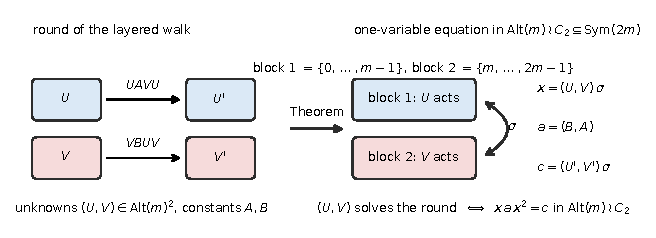
\includegraphics[width=\textwidth]{fig_wreath}
\caption{The wreath normal form (Theorem~\ref{thm:wreath}). Left: one round of the layered walk, with registers $U,V\in\Alt(m)$ and public constants $A,B$. Right: the same round as the single equation $x\,a\,x^{2}=c$ in $\Alt(m)\wr C_2\le\Sym(2m)$, where the base group acts blockwise and $\sigma$ swaps the two blocks. The unknown $x$ and the target $c$ lie in the coset $(\Alt(m)\times\Alt(m))\sigma$; the constant $a=(B,A)$ lies in the base group.}
\label{fig:wreath}
\end{figure}

\begin{thm}[wreath normal form]\label{thm:wreath}
Let $K=(\Alt(m)\times\Alt(m))\rtimes C_2=\Alt(m)\wr C_2\le\Sym(2m)$, where $(U,V)$ acts on $\{0,\ldots,m-1\}$ by $U$ and on $\{m,\ldots,2m-1\}$ by $V$, and $\sigma$ swaps the two blocks. Put $x=(U,V)\sigma$, $a=(B,A)$, $c=(U',V')\sigma$. Then $(U,V)$ solves $\mathcal R(U',V';A,B)$ iff $x\,a\,x^{2}=c$ in $K$, and every solution of this equation in $K$ is of the form $(U,V)\sigma$. The single-round system is thus $\Pthree$ in the subgroup $K$.
\end{thm}
\begin{proof}
In $K$, $\sigma(P,Q)\sigma^{-1}=(Q,P)$. With $g=(U,V)$,
\begin{align*}(g\sigma)\,a\,(g\sigma)(g\sigma)&=g\,(\sigma a\sigma^{-1})(\sigma g\sigma^{-1})\,g\,\sigma\\&=(U,V)(A,B)(V,U)(U,V)\sigma=(UAVU,\,VBUV)\sigma,\end{align*}
which equals $c$ iff \eqref{eq:round} holds. Since $a$ is in the base group and $c$ in the non-trivial coset, $xax^{2}\in(\Alt(m)\times\Alt(m))\sigma$ forces $x$ into that coset.
\end{proof}
Verified exhaustively at $m=5$ (all $3600$ pairs $(U,V)$ for $21$ pairs $(A,B)$) and on $3000$ random instances at each of $m=6,7$. Three remarks. (i) The elimination of $V$ from \eqref{eq:round} gives a one-unknown equation with five occurrences of $U$ (three positive, two negative); the wreath form has three positive occurrences and one constant. (ii) The case $a=1$, i.e.\ $A=B=1$, is the cube root $x^{3}=c$ and is polynomial. (iii) The relaxation of $xax^{2}=c$ from $K$ to $\Sym(2m)$ is \emph{not} equivalent to the round system: on planted instances at $m=5$ it acquires solutions outside $\Sym(m)\wr C_2$, so any solver for the round must keep the block structure. By the conjugation normal form $(U,V)\mapsto(Ug,g^{-1}V)$, $(A,B)\mapsto(g^{-1}Ag,B)$, the difficulty of a round depends on $(A,B)$ only through their conjugacy classes; no degenerate choice ($A=B$, $A=B^{-1}$, commuting $A,B$, $A$ of order two, $U'=V'$) was found to reduce the round to roots or conjugacy except $A=B=1$ (exhaustive at $m=5$).

\subsection{The cost of constraint propagation}

The natural solver works on the pointwise form $c(j)=x(a(x(x(j))))$: for every point $j$ the chain $j\to x(j)\to x^{2}(j)\to a x^{2}(j)\to c(j)$ contains three applications of $x$, and a chain forces its missing letter as soon as the other two are known. The solver propagates to a fixed point after every assignment and branches on an undetermined image; its cost is counted in search nodes, a machine-independent unit. Two branching rules were measured: the first free point, and the point with the fewest surviving images under one step of propagation (``most constrained first''). Instances are planted, $x$ uniform in the coset, $(A,B)$ uniform in $\Alt(m)^{2}$, five instances per degree, seeds derived by SHA-256 from labelled strings.

\begin{obs}[cost law]\label{obs:cost}
On $m=5,\ldots,16$ (Figure~\ref{fig:cost}b) the planted solution is reached after $k(m)\approx0.38\,m+0.6$ free decisions, each with a domain of about $m$ values, after which propagation completes the assignment; the first decision never propagates, the cascade occurs at decision $3$--$7$, wrong branches are refuted at the same depth as the right one, and $90$--$95\%$ of the nodes hang below the wrong children of the root. A random-coverage model (reveal $k$ images, propagate) reproduces the tree size within $30\%$. Hence $\log_2(\text{nodes})\approx(0.38\,m+0.6)\log_2(0.7\,m)+O(1)$: the cost is $|\Alt(m)|^{\Theta(1)}$ with exponent between one fifth and two fifths of brute force ($\log_2|\Alt(m)|\approx m\log_2m-1.44m$;
coefficients $0.22$ and $0.37$ in Table~\ref{tab:cost}), and any linear fit in bits per unit of degree is its tangent in the measured window.
\end{obs}
\begin{figure}[htbp]\centering
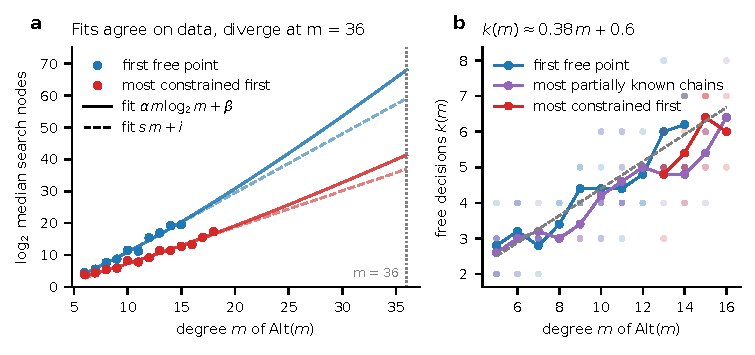
\includegraphics[width=\textwidth]{fig_cost_law}
\caption{Cost of the propagation solver on planted wreath instances, five instances per degree. (a) $\log_2$ of the median number of search nodes to the first solution for the two branching rules, with the linear and the $\alpha\,m\log_2 m$ fits of Table~\ref{tab:cost}; the two models coincide on the measured window and diverge at the originally proposed degree $m=36$. (b) Number $k(m)$ of free decisions before propagation completes the planted solution, for three branching rules (small dots: individual instances; large dots: means; dashed: $0.38\,m+0.6$). Each free decision has a domain of about $m$ values, which gives the $m\log m$ exponent.}
\label{fig:cost}
\end{figure}

The mechanism is the peeling threshold of the constraint hypergraph: $N$ chains, $N$ unknown images, three letters per chain; a cascade requires a seed of linear size, since a single known image never completes two letters of any chain.

\begin{table}[htbp]\centering
\caption{Fitted cost of the propagation solver on wreath instances, $\log_2$ of the median number of search nodes to the first solution, five planted instances per degree, fitted on the degree window given under each rule. Both models fit the window equally; they diverge beyond it, so extrapolations are reported as intervals. All entries are $\log_2$ values; the last column is the combined attack cost $2^{n/2}\TR(m)$ at $(n,m)=(256,36)$.}\label{tab:cost}
\footnotesize\setlength{\tabcolsep}{3.5pt}
\begin{tabular}{@{}llrccc@{}}\toprule
Branching rule & Model & Fit & $\TR(36)$ & $\TR(48)$ & attack\\\midrule
first free point & linear & $1.85\,m-7.53$ & $59$ & $81$ & $187$\\
 ($m=8$--$15$) & $m\log m$ & $0.374\,m\log_2 m-1.52$ & $68$ & $99$ & $196$\\[2pt]
most constrained first & linear & $1.14\,m-4.10$ & $37$ & $51$ & $165$\\
 ($m=8$--$18$) & $m\log m$ & $0.223\,m\log_2 m-0.13$ & $41$ & $60$ & $169$\\
\bottomrule\end{tabular}
\end{table}

\begin{figure}[htbp]\centering
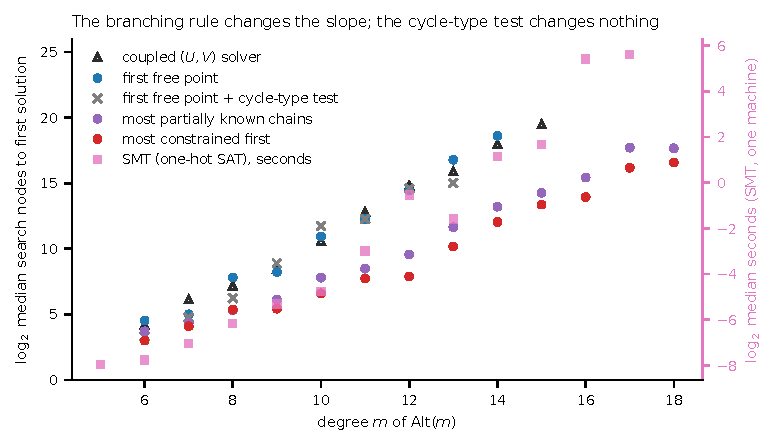
\includegraphics[width=\textwidth]{fig_variants}
\caption{Solver variants on planted wreath instances, $\log_2$ of the median number of search nodes to the first solution ($5$--$9$ instances per degree). The branching rule changes the slope of the cost curve (first free point against most constrained first); adding the cycle-type test $\ctype(ax^{3})=\ctype(c)$ to propagation changes nothing, since the test is implied by the local constraints. The coupled $(U,V)$ solver of the original construction and the wreath-form solver with the same branching rule coincide. The SMT encoding (one-hot SAT, right axis, seconds on one machine) has the same exponent.}
\label{fig:var}
\end{figure}

Table~\ref{tab:cost} and Figures~\ref{fig:cost}a and~\ref{fig:var} give the two fits and the variant comparison. The most-constrained rule lowers the coefficient of the $m\log m$ law from $0.37$ to $0.22$, not merely a constant: $15$--$55$ times fewer nodes at $m=13$--$16$. A cycle-type relaxation of $\ctype(ax^{3})=\ctype(c)$ never pruned a node (it is implied by the local constraints); a one-hot SAT encoding solved by a modern SMT solver has the same exponent and is $10$--$20$ times slower in wall time; the conjugated form $x^{3}=a^{-1}y$, $y\sim c$, reduces to enumerating the class of $c$ and is not competitive. Generic instances in $\Sym(N)$ without block structure cost the same as wreath instances ($1.20$ against $1.23$ bits per point of $N$, $N=14$--$22$): the difficulty is that of $\Pthree$, not of the subgroup.

Read at the parameters originally proposed, $(n,m)=(256,36)$, the attack costs between $2^{165}$ and $2^{196}$ depending on the branching rule and the cost model -- far below the $2^{256}$ of exhaustive search, far above the $2^{128}$ target. The parameters are not broken; but the whole margin is the factor $2^{n/2}$, which a meet-in-the-middle attack makes necessary rather than surplus, and a better round solver raises the degree a sizing rule must require (if the rule requires $\TR(m)\ge2^{128}$: from $m=59$--$74$ with the first-free-point fits to $m=89$--$116$ with the most-constrained fits of
Table~\ref{tab:cost}, the lower value of each pair coming from the $m\log m$ model). Only a lower bound for $\Pthree$ would let it fall back to the capacity value $m=36$.

\section{Open problems}\label{sec:open}
\begin{enumerate}
\item Is $\Pthree$ -- the equation $x\,a\,x^{2}=c$ over $\Sym(N)$ -- NP-complete, or in P, or neither? By Lemma~\ref{lem:twoeq} the NP-complete problem $\Dzero$ is the system of the two equations $xax^{2}=c$, $xa^{2}x^{2}=c^{2}$; the question is whether one equation can simulate the pair. Disjoint padding and layered paddings cannot (Remark~\ref{rem:padding}, Proposition~\ref{prop:fourlayer}), and any hardness proof must use solutions moving the constant (Remark~\ref{rem:notproved}).
\item Is $\Pthree^{\lambda}$ NP-complete for every $\lambda$ of unbounded support with a part at least $4$, in particular for $\lambda=(N)$? For such $\lambda$ no polynomial criterion was found at $N\le9$; for all parts coprime to $3$, $\Pthree^{\lambda}$ asks whether $c=z^{k}az^{1-k}$ for some $z$ of type $\lambda$, $k\equiv3^{-1}\pmod{\operatorname{lcm}\lambda}$.
\item Is there a polynomial-time algorithm for $\Pthree$ when $a$ is an $N$-cycle (equivalently, by Proposition~\ref{prop:dual}, when $c$ is)? Theorem~\ref{thm:transposition} settles transposition targets; the solvable set is invariant under $\langle a\rangle$ only, so a criterion cannot be reflection-symmetric.
\item Is the solution count $\#\{x:xax^{2}=c\}$ computable in polynomial time, or $\#\mathrm P$-hard? Only its first moment over a class is known in closed form (Theorem~\ref{thm:firstmoment}); the count restricted to solutions of order three is at least as hard as counting the solutions of N3DM: in the reduction of
Theorem~\ref{thm:main} every admissible triple admits exactly $L^{2}$ translation vectors, so the number of order-three conjugators is
$L^{2q}$ times the number of matchings.
\item Is there a reduction for $\Conj{n}$ that is polynomial in $n$ when $n$ is part of the input (the reduction of Theorem~\ref{thm:conjn} has size $\Theta(qB'(n+1)^{n-1})$)? Does hardness survive when the cycle length $L$ of $a$ is fixed rather than growing with the instance? And for which cycle types $\lambda$ other than $n^{N/n}$ is ``conjugacy by an element of type $\lambda$'' NP-complete -- in particular for fixed-point-free involutions?
\item Is the $|\Alt(m)|^{\Theta(1)}$ cost of Observation~\ref{obs:cost} a lower bound for all local-propagation solvers, via the peeling threshold?
\item Do the mixed-sign words of $x$-length three, such as $x\,a\,x\,b\,x^{-1}=c$, reduce to $\Pthree$, to conjugacy, or to something else?
\end{enumerate}

\section*{Reproducibility} The exhaustive and randomised checks cited above were produced by Python scripts (standard library; numpy for the exhaustive tables) that are archived, with their recorded outputs, in the repository \url{https://github.com/gautierfilardo-efrei/order3-conjugacy} (release \texttt{v0.4.0}); the round solver and cost records of Section~\ref{sec:cpwi} are released with \cite{filardo2026cpwi} (release \texttt{v1.3.0}). Timings are local; all reported costs are search-node counts.

\section*{Acknowledgements} Generative AI tools assisted with code development and text drafting; the mathematics, sources and interpretation were reviewed by the author.

\bibliographystyle{elsarticle-num}
\bibliography{p3_refs}
\end{document}
